\documentclass[a4paper,11pt]{article}
\usepackage[verbose,a4paper,tmargin=2cm,bmargin=2cm,lmargin=2.5cm,rmargin=2.5cm]{geometry}
\usepackage{polski}
\usepackage{amsmath}
\usepackage{amsfonts}
\usepackage{amssymb}
\usepackage{lastpage}
\usepackage{indentfirst}
\usepackage{verbatim}
\usepackage{graphicx}
\usepackage{fancyhdr}
\usepackage{listings}
\usepackage{float}
\usepackage{hyperref}
\hypersetup{
    colorlinks = true,
    linkcolor = black,
    urlcolor = cyan
}
\usepackage{xcolor}
\usepackage{tikz}
\usepackage{multirow}
\frenchspacing
\pagestyle{fancyplain}
\fancyhf{}

\usepackage{setspace}
\usepackage{enumitem}

\renewcommand{\headrulewidth}{0pt}
\renewcommand{\footrulewidth}{0.4pt}
\newcommand{\degree}{\ensuremath{^{\circ}}} 
\fancyfoot[L]{MUM: P. Galewicz, B. Jurczewski, Z. Nowacki, K.Podlewski, P. Wardęcki}
\fancyfoot[R]{\thepage\ / \pageref{LastPage}}

\begin{document}

%%%%%%%%%%%%%%%%%%%%%%%%%%%%%%%%%%%%%%%%%%%% STRONA TYTUŁOWA

\begin{titlepage}
\begin{center}
\begin{tabular}{rcl}
\begin{tabular}{|r|}
\hline \\
\large{\underline{234053~~~~~~~~~~~~~~~~~~~~~~~} }\\
\small{\textit{Numer indeksu}}\\
\large{\underline{Paweł Galewicz~~~~~~~~~~~~} }\\
\small{\textit{Imię i nazwisko}}\\\\ \hline
\end{tabular} 
&
\begin{tabular}{|r|}
\hline \\
\large{\underline{234067~~~~~~~~~~~~~~~~~~~~~~~} }\\
\small{\textit{Numer indeksu}}\\
\large{\underline{Bartosz Jurczewski~~~~~~~} }\\
\small{\textit{Imię i nazwisko}}\\\\ \hline
\end{tabular} 
&
\begin{tabular}{|r|}
\hline \\
\large{\underline{234102~~~~~~~~~~~~~~~~~~~~~~~} }\\
\small{\textit{Numer indeksu}}\\
\large{\underline{Zbigniew Nowacki~~~~~~~~} }\\
\small{\textit{Imię i nazwisko}}\\\\ \hline
\end{tabular} 
\end{tabular} 

\vspace{10px}

\begin{tabular}{rl}
\begin{tabular}{|r|}
\hline \\
\large{\underline{234106~~~~~~~~~~~~~~~~~~~~~~~} }\\
\small{\textit{Numer indeksu}}\\
\large{\underline{Karol Podlewski~~~~~~~~~~~} }\\
\small{\textit{Imię i nazwisko}}\\\\ \hline
\end{tabular} 
&
\begin{tabular}{|r|}
\hline \\
\large{\underline{234128~~~~~~~~~~~~~~~~~~~~~~~} }\\
\small{\textit{Numer indeksu}}\\
\large{\underline{Piotr Wardęcki~~~~~~~~~~~~} }\\
\small{\textit{Imię i nazwisko}}\\\\ \hline
\end{tabular} 
\end{tabular}
\end{center}

\vspace{25px}

\begin{tabular}{ll}
\LARGE{\textbf{Kierunek}}& \LARGE{Informatyka Stosowana} \\
\LARGE{\textbf{Stopień}}& \LARGE{II} \\
\LARGE{\textbf{Specjalizacja}}& \LARGE{Data Science} \\
\LARGE{\textbf{Semestr}}& \LARGE{1} \\\\
\LARGE{\textbf{Data oddania}}& \LARGE{6 maja 2020} \\\\\\\\\\\\\\
\end{tabular}

\begin{center}
\textbf{\huge{\\~\\Metody uczenia maszynowego }}
\textbf{\Huge{\\~\\Problem set 3}}
\end{center}

\end{titlepage}

\setcounter{page}{2}
\setstretch{1.5}
\tableofcontents
\newpage
\setstretch{1.1}

%%%%%%%%%%%%%%%%%%%%%%%%%%%%%%%%%%%%%%%%%%%% CEL

\section{Cel} \label{sec:cel}
Zadanie polegało na ocenie jakości modeli, które przygotowane były w poprzednich zadaniach -- klasyfikacji oraz analizy skupień. Do oceny tej wykonane zostały różne testy z wykorzystaniem odpowiednich miar ewaluacyjnych oraz metod walidacji.

%%%%%%%%%%%%%%%%%%%%%%%%%%%%%%%%%%%%%%%%%%%% OPIS IMPLEMENTACJI

\section{Opis implementacji}
Algorytmy oraz przygotowane do nich testy zostały zaimplementowane za pomocą języka Python w wersji 3.8.2.
Wykorzystano w nim biblioteki NumPy, Sklearn i Pandas. 

%%%%%%%%%%%%%%%%%%%%%%%%%%%%%%%%%%%%%%%%%%%% OPIS ZBIORÓW DANYCH

\section{Opis zbiorów danych} \label{sec:dataset}

\subsection{Klasyfikacja}

Bazowaliśmy na trzech zestawach danych, przeznaczonych do klasyfikacji binarnej: 

\begin{enumerate}[label=\Alph*.] \label{zbiory_klasyfikacja}
    \item{\href{https://www.kaggle.com/bobbyscience/league-of-legends-diamond-ranked-games-10-min}{League of Legends Diamond Ranked Games (10 min)}} -- zbiór zawierający dane dotyczące meczy rankingowych na wysokim poziomie w grze League of Legends, składający się z 38 cech, po 19 dla każdej drużyny. Zebrane wartości to informacje o między innymi zgromadzonym złocie, zniszczonych wieżach, zgładzonych potworach czy przeciwnikach na przestrzeni pierwszych 10 minut mapy. Do cech tych przypisana jest informacja o zwycięstwie danej drużyny. 
    \item{\href{https://www.kaggle.com/jsphyg/weather-dataset-rattle-package}{Rain in Australia}} -- historia danych pogodowych z 10 lat (data, lokalizacja, temperatury, opady, wiatr, ciśnienie, wilgotność, nasłonecznienie itp). Na podstawie 23 cech należy określić, czy kolejnego dnia wystąpią opady.
    \item{\href{https://www.kaggle.com/uciml/pima-indians-diabetes-database}{Pima Indians Diabetes Database}} -- zbiór danych zawierający 8 niepowiązanych ze sobą pomiarów diagnostycznych (m. in. ilość ciąż, poziom glukozy, ciśnienie, bmi, wiek) na podstawie których dokonywana jest ocena, czy kobieta choruje na cukrzycę.
\end{enumerate}

\subsection{Klasteryzacja}

Bazowaliśmy na trzech zestawach danych: 

\begin{enumerate}[label=\Alph*.] \label{zbiory_klasteryzacja}
    \item{\href{https://www.kaggle.com/vjchoudhary7/customer-segmentation-tutorial-in-python}{Mall Customer Segmentation}} - Zawiera informacje zbierane od klientów centrum handlowego uczestniczących w programie lojalnościowym. Są to między innymi dane o wieku, płci, rocznym przychodzie. Każdy klient ma też wyliczoną ocenę wydatków w sklepie w przedziale od 1 do 100.
    \item{\href{https://www.kaggle.com/maitree/wine-quality-selection#winequality-red.csv}{Wine quality selection}} -- Zestaw danych przedstawiający współczynniki wina wraz z przyporządkowaną ich jakością.
    \item{\href{https://www.kaggle.com/arjunbhasin2013/ccdata}{Credit Card Dataset}} -- Zbiór opisujący zachowania aktywnych klientów bankowych, agregowanych przez 6miesięcy.
\end{enumerate}

%%%%%%%%%%%%%%%%%%%%%%%%%%%%%%%%%%%%%%%%%%%% EWALUACJA KLASYFIKACJI

\section{Ewaluacja modeli klasyfikacyjnych}
Model klasyfikacji przygotowany został w ramach zadania 1. Zawiera on implementacje następujących metod:

\begin{enumerate}
    \item Algorytm drzew decyzyjnych
    \item Naiwny klasyfikator Bayesa
    \item Maszyna wektorów nośnych
    \item Klasyfikator k-najbliższych sąsiadów
    \item Algorytm sztucznych sieci neuronowych
\end{enumerate}

Na każdej z metod przeprowadzone zostały testy, które miały na celu sprawdzenie jak dobrze spełniają one swoje zadanie. Za każdym razem wykorzystano 75\% danych jako część treningową.

%%%%%%%%%%%%%%%%%%%%%% Macierz pomyłek 

\subsection{Wartości podstawowych metryk ewaluacyjnych}
Pierwszy test zakładał stworzenie macierzy pomyłek dla każdej metody klasyfikacji i na jej podstawie wyliczenie podstawowych metryk ewaluacyjnych: 
\begin{itemize}
    \item Dokładność -- Określa jak duży odsetek obserwacji został prawidłowo zaklasyfikowany.
    \item Precyzja -- Oznacza jak dużo zaklasyfikowanych do danej klasy obserwacji rzeczywiście do niej należy. 
    \item Czułość -- Stosunek liczby obserwacji oznaczonych jako \textit{true positive} do sumy \textit{true positive} i \textit{false negative}. Jej wartość interpretować można jako zdolność do prawidłowego zakwalifikowania obserwacji do odpowiedniej klasy. 
    \item Specyficzność -- Stosunek liczby obserwacji \textit{true negative} do sumy \textit{true negative} i \textit{false positive}. Określa jak dobrze model rozpoznaje, że dana obserwacja nie należy do danej klasy.
\end{itemize} 


%%%%%%%%%%% Zbiór A
\subsubsection*{Zbiór A}

\begin{table}[H]
\centering
\caption{Macierz pomyłek dla algorytmu drzew decyzyjnych, dla zbioru A}
\label{tab:con_mat_1a}
\begin{tabular}{c|c|c|c|}
\cline{3-4}
\multicolumn{2}{c|}{\multirow{2}{*}{\textbf{}}} & \multicolumn{2}{c|}{\textbf{Klasa predykowana}} \\ \cline{3-4} 
\multicolumn{2}{c|}{} & \textbf{Pozytywna} & \multicolumn{1}{l|}{\textbf{Negatywna}} \\ \hline
\multicolumn{1}{|c|}{\multirow{2}{*}{\textbf{\begin{tabular}[c]{@{}c@{}}Klasa\\ rzeczywista\end{tabular}}}} & \textbf{Pozytywna} & 785 & 461 \\ \cline{2-4} 
\multicolumn{1}{|c|}{} & \textbf{Negatywna} & 457 & 766 \\ \hline
\end{tabular}
\end{table}

\begin{table}[H]
\centering
\caption{Macierz pomyłek dla naiwnego klasyfikatora Bayesa, dla zbioru A}
\label{tab:con_mat_2a}
\begin{tabular}{c|c|c|c|}
\cline{3-4}
\multicolumn{2}{c|}{\multirow{2}{*}{\textbf{}}} & \multicolumn{2}{c|}{\textbf{Klasa predykowana}} \\ \cline{3-4} 
\multicolumn{2}{c|}{} & \textbf{Pozytywna} & \multicolumn{1}{l|}{\textbf{Negatywna}} \\ \hline
\multicolumn{1}{|c|}{\multirow{2}{*}{\textbf{\begin{tabular}[c]{@{}c@{}}Klasa\\ rzeczywista\end{tabular}}}} & \textbf{Pozytywna} & 879 & 338 \\ \cline{2-4} 
\multicolumn{1}{|c|}{} & \textbf{Negatywna} & 331 & 921 \\ \hline
\end{tabular}
\end{table}

\begin{table}[H]
\centering
\caption{Macierz pomyłek dla maszyny wektorów nośnych, dla zbioru A}
\label{tab:con_mat_3a}
\begin{tabular}{c|c|c|c|}
\cline{3-4}
\multicolumn{2}{c|}{\multirow{2}{*}{\textbf{}}} & \multicolumn{2}{c|}{\textbf{Klasa predykowana}} \\ \cline{3-4} 
\multicolumn{2}{c|}{} & \textbf{Pozytywna} & \multicolumn{1}{l|}{\textbf{Negatywna}} \\ \hline
\multicolumn{1}{|c|}{\multirow{2}{*}{\textbf{\begin{tabular}[c]{@{}c@{}}Klasa\\ rzeczywista\end{tabular}}}} & \textbf{Pozytywna} & 889 & 378 \\ \cline{2-4} 
\multicolumn{1}{|c|}{} & \textbf{Negatywna} & 304 & 898 \\ \hline
\end{tabular}
\end{table}

\begin{table}[H]
\centering
\caption{Macierz pomyłek dla klasyfikatora k-nn, dla zbioru A}
\label{tab:con_mat_4a}
\begin{tabular}{c|c|c|c|}
\cline{3-4}
\multicolumn{2}{c|}{\multirow{2}{*}{\textbf{}}} & \multicolumn{2}{c|}{\textbf{Klasa predykowana}} \\ \cline{3-4} 
\multicolumn{2}{c|}{} & \multicolumn{1}{c|}{\textbf{Pozytywna}} & \textbf{Negatywna} \\ \hline
\multicolumn{1}{|c|}{\multirow{2}{*}{\textbf{\begin{tabular}[c]{@{}c@{}}Klasa\\ rzeczywista\end{tabular}}}} & \textbf{Pozytywna} & 832 & 411 \\ \cline{2-4} 
\multicolumn{1}{|c|}{} & \textbf{Negatywna} & 373 & 853 \\ \hline
\end{tabular}
\end{table}

\begin{table}[H]
\centering
\caption{Macierz pomyłek dla sztucznej sieci neuronowej, dla zbioru A}
\label{tab:con_mat_5a}
\begin{tabular}{c|c|c|c|}
\cline{3-4}
\multicolumn{2}{c|}{\multirow{2}{*}{\textbf{}}} & \multicolumn{2}{c|}{\textbf{Klasa predykowana}} \\ \cline{3-4} 
\multicolumn{2}{c|}{} & \textbf{Pozytywna} & \multicolumn{1}{l|}{\textbf{Negatywna}} \\ \hline
\multicolumn{1}{|c|}{\multirow{2}{*}{\textbf{\begin{tabular}[c]{@{}c@{}}Klasa\\ rzeczywista\end{tabular}}}} & \textbf{Pozytywna} & 1207 & 22 \\ \cline{2-4} 
\multicolumn{1}{|c|}{} & \textbf{Negatywna} & 1079 & 161 \\ \hline
\end{tabular}
\end{table}

\begin{table}[H]
\centering
\caption{Wartości metryk ewaluacyjnych dla zbioru A}
\label{tab:metrics_a}
\begin{tabular}{|l|c|c|c|c|}
\hline
\multicolumn{1}{|c|}{\textbf{Algorytm}} & \textbf{Precyzja} & \textbf{Dokładność} & \textbf{Czułość} & \textbf{Specyficzność} \\ \hline
Drzew decyzyjnych & 0.632 & 0.628 & 0.63 & 0.626 \\ \hline
Naiwny klasyfikator Bayesa & 0.726 & 0.729 & 0.722 & 0.736 \\ \hline
Maszyna wektorów nośnych & 0.745 & 0.724 & 0.702 & 0.747 \\ \hline
Klasyfikator k-nn & 0.69 & 0.682 & 0.669 & 0.696 \\ \hline
Sztucznych sieci neuronowych & 0.528 & 0.554 & 0.982 & 0.13 \\ \hline
\end{tabular}
\end{table}

%%%%%%%%%%% Zbiór B
\subsubsection*{Zbiór B}

\begin{table}[H]
\centering
\caption{Macierz pomyłek dla algorytmu drzew decyzyjnych, dla zbioru B}
\label{tab:con_mat_1b}
\begin{tabular}{c|c|c|c|}
\cline{3-4}
\multicolumn{2}{c|}{\multirow{2}{*}{\textbf{}}} & \multicolumn{2}{c|}{\textbf{Klasa predykowana}} \\ \cline{3-4} 
\multicolumn{2}{c|}{} & \textbf{Pozytywna} & \textbf{Negatywna} \\ \hline
\multicolumn{1}{|c|}{\multirow{2}{*}{\textbf{\begin{tabular}[c]{@{}c@{}}Klasa\\ rzeczywista\end{tabular}}}} & \textbf{Pozytywna} & 3115 & 0 \\ \cline{2-4} 
\multicolumn{1}{|c|}{} & \textbf{Negatywna} & 0 & 10989 \\ \hline
\end{tabular}
\end{table}

\begin{table}[H]
\centering
\caption{Macierz pomyłek dla naiwnego klasyfikatora Bayesa, dla zbioru B}
\label{tab:con_mat_2b}
\begin{tabular}{c|c|c|c|}
\cline{3-4}
\multicolumn{2}{c|}{\multirow{2}{*}{\textbf{}}} & \multicolumn{2}{c|}{\textbf{Klasa predykowana}} \\ \cline{3-4} 
\multicolumn{2}{c|}{} & \textbf{Pozytywna} & \textbf{Negatywna} \\ \hline
\multicolumn{1}{|c|}{\multirow{2}{*}{\textbf{\begin{tabular}[c]{@{}c@{}}Klasa\\ rzeczywista\end{tabular}}}} & \textbf{Pozytywna} & 3036 & 1 \\ \cline{2-4} 
\multicolumn{1}{|c|}{} & \textbf{Negatywna} & 812 & 10255 \\ \hline
\end{tabular}
\end{table}

\begin{table}[H]
\centering
\caption{Macierz pomyłek dla maszyny wektorów nośnych, dla zbioru B}
\label{tab:con_mat_3b}
\begin{tabular}{c|c|c|c|}
\cline{3-4}
\multicolumn{2}{c|}{\multirow{2}{*}{\textbf{}}} & \multicolumn{2}{c|}{\textbf{Klasa predykowana}} \\ \cline{3-4} 
\multicolumn{2}{c|}{} & \textbf{Pozytywna} & \textbf{Negatywna} \\ \hline
\multicolumn{1}{|c|}{\multirow{2}{*}{\textbf{\begin{tabular}[c]{@{}c@{}}Klasa\\ rzeczywista\end{tabular}}}} & \textbf{Pozytywna} & 485 & 2644 \\ \cline{2-4} 
\multicolumn{1}{|c|}{} & \textbf{Negatywna} & 1 & 10974 \\ \hline
\end{tabular}
\end{table}

\begin{table}[H]
\centering
\caption{Macierz pomyłek dla klasyfikatora k-nn, dla zbioru B}
\label{tab:con_mat_4b}
\begin{tabular}{c|c|c|c|}
\cline{3-4}
\multicolumn{2}{c|}{\multirow{2}{*}{\textbf{}}} & \multicolumn{2}{c|}{\textbf{Klasa predykowana}} \\ \cline{3-4} 
\multicolumn{2}{c|}{} & \textbf{Pozytywna} & \textbf{Negatywna} \\ \hline
\multicolumn{1}{|c|}{\multirow{2}{*}{\textbf{\begin{tabular}[c]{@{}c@{}}Klasa\\ rzeczywista\end{tabular}}}} & \textbf{Pozytywna} & 1589 & 1497 \\ \cline{2-4} 
\multicolumn{1}{|c|}{} & \textbf{Negatywna} & 405 & 10613 \\ \hline
\end{tabular}
\end{table}

\begin{table}[H]
\centering
\caption{Macierz pomyłek dla sztucznej sieci neuronowej, dla zbioru B}
\label{tab:con_mat_5b}
\begin{tabular}{c|c|c|c|}
\cline{3-4}
\multicolumn{2}{c|}{\multirow{2}{*}{\textbf{}}} & \multicolumn{2}{c|}{\textbf{Klasa predykowana}} \\ \cline{3-4} 
\multicolumn{2}{c|}{} & \textbf{Pozytywna} & \textbf{Negatywna} \\ \hline
\multicolumn{1}{|c|}{\multirow{2}{*}{\textbf{\begin{tabular}[c]{@{}c@{}}Klasa\\ rzeczywista\end{tabular}}}} & \textbf{Pozytywna} & 3108 & 6 \\ \cline{2-4} 
\multicolumn{1}{|c|}{} & \textbf{Negatywna} & 147 & 10843 \\ \hline
\end{tabular}
\end{table}

\begin{table}[H]
\centering
\caption{Wartości metryk ewaluacyjnych dla zbioru B}
\label{tab:metrics_b}
\begin{tabular}{|l|c|c|c|c|}
\hline
\multicolumn{1}{|c|}{\textbf{Algorytm}} & \textbf{Precyzja} & \textbf{Dokładność} & \textbf{Czułość} & \textbf{Specyficzność} \\ \hline
Drzew decyzyjnych & 1.0 & 1.0 & 1.0 & 1.0 \\ \hline
Naiwny klasyfikator Bayesa & 0.789 & 0.942 & 1.0 & 0.927 \\ \hline
Maszyna wektorów nośnych & 0.998 & 0.812 & 0.155 & 1.0 \\ \hline
Klasyfikator k-nn & 0.797 & 0.865 & 0.515 & 0.963 \\ \hline
Sztucznych sieci neuronowych & 0.955 & 0.989 & 0.998 & 0.987 \\ \hline
\end{tabular}
\end{table}

%%%%%%%%%%% Zbiór C
\subsubsection*{Zbiór C}

\begin{table}[H]
\centering
\caption{Macierz pomyłek dla algorytmu drzew decyzyjnych, dla zbioru C}
\label{tab:con_mat_1c}
\begin{tabular}{c|c|c|c|}
\cline{3-4}
\multicolumn{2}{c|}{\multirow{2}{*}{\textbf{}}} & \multicolumn{2}{c|}{\textbf{Klasa predykowana}} \\ \cline{3-4} 
\multicolumn{2}{c|}{} & \textbf{Pozytywna} & \multicolumn{1}{l|}{\textbf{Negatywna}} \\ \hline
\multicolumn{1}{|c|}{\multirow{2}{*}{\textbf{\begin{tabular}[c]{@{}c@{}}Klasa\\ rzeczywista\end{tabular}}}} & \textbf{Pozytywna} & 40 & 30 \\ \cline{2-4} 
\multicolumn{1}{|c|}{} & \textbf{Negatywna} & 24 & 97 \\ \hline
\end{tabular}
\end{table}

\begin{table}[H]
\centering
\caption{Macierz pomyłek dla naiwnego klasyfikatora Bayesa, dla zbioru C}
\label{tab:con_mat_2c}
\begin{tabular}{c|c|c|c|}
\cline{3-4}
\multicolumn{2}{c|}{\multirow{2}{*}{\textbf{}}} & \multicolumn{2}{c|}{\textbf{Klasa predykowana}} \\ \cline{3-4} 
\multicolumn{2}{c|}{} & \textbf{Pozytywna} & \multicolumn{1}{l|}{\textbf{Negatywna}} \\ \hline
\multicolumn{1}{|c|}{\multirow{2}{*}{\textbf{\begin{tabular}[c]{@{}c@{}}Klasa\\ rzeczywista\end{tabular}}}} & \textbf{Pozytywna} & 36 & 33 \\ \cline{2-4} 
\multicolumn{1}{|c|}{} & \textbf{Negatywna} & 20 & 102 \\ \hline
\end{tabular}
\end{table}

\begin{table}[H]
\centering
\caption{Macierz pomyłek dla maszyny wektorów nośnych, dla zbioru C}
\label{tab:con_mat_3c}
\begin{tabular}{c|c|c|c|}
\cline{3-4}
\multicolumn{2}{c|}{\multirow{2}{*}{\textbf{}}} & \multicolumn{2}{c|}{\textbf{Klasa predykowana}} \\ \cline{3-4} 
\multicolumn{2}{c|}{} & \textbf{Pozytywna} & \multicolumn{1}{l|}{\textbf{Negatywna}} \\ \hline
\multicolumn{1}{|c|}{\multirow{2}{*}{\textbf{\begin{tabular}[c]{@{}c@{}}Klasa\\ rzeczywista\end{tabular}}}} & \textbf{Pozytywna} & 36 & 29 \\ \cline{2-4} 
\multicolumn{1}{|c|}{} & \textbf{Negatywna} & 10 & 116 \\ \hline
\end{tabular}
\end{table}

\begin{table}[H]
\centering
\caption{Macierz pomyłek dla klasyfikatora k-nn, dla zbioru C}
\label{tab:con_mat_4c}
\begin{tabular}{c|c|c|c|}
\cline{3-4}
\multicolumn{2}{c|}{\multirow{2}{*}{\textbf{}}} & \multicolumn{2}{c|}{\textbf{Klasa predykowana}} \\ \cline{3-4} 
\multicolumn{2}{c|}{} & \textbf{Pozytywna} & \multicolumn{1}{l|}{\textbf{Negatywna}} \\ \hline
\multicolumn{1}{|c|}{\multirow{2}{*}{\textbf{\begin{tabular}[c]{@{}c@{}}Klasa\\ rzeczywista\end{tabular}}}} & \textbf{Pozytywna} & 39 & 29 \\ \cline{2-4} 
\multicolumn{1}{|c|}{} & \textbf{Negatywna} & 23 & 100 \\ \hline
\end{tabular}
\end{table}

\begin{table}[H]
\centering
\caption{Macierz pomyłek dla sztucznej sieci neuronowej, dla zbioru C}
\label{tab:con_mat_5c}
\begin{tabular}{c|c|c|c|}
\cline{3-4}
\multicolumn{2}{c|}{\multirow{2}{*}{\textbf{}}} & \multicolumn{2}{c|}{\textbf{Klasa predykowana}} \\ \cline{3-4} 
\multicolumn{2}{c|}{} & \textbf{Pozytywna} & \multicolumn{1}{l|}{\textbf{Negatywna}} \\ \hline
\multicolumn{1}{|c|}{\multirow{2}{*}{\textbf{\begin{tabular}[c]{@{}c@{}}Klasa\\ rzeczywista\end{tabular}}}} & \textbf{Pozytywna} & 41 & 14 \\ \cline{2-4} 
\multicolumn{1}{|c|}{} & \textbf{Negatywna} & 40 & 96 \\ \hline
\end{tabular}
\end{table}

\begin{table}[H]
\centering
\caption{Wartości metryk ewaluacyjnych dla zbioru C}
\label{tab:metrics_c}
\begin{tabular}{|l|c|c|c|c|}
\hline
\multicolumn{1}{|c|}{\textbf{Algorytm}} & \textbf{Precyzja} & \textbf{Dokładność} & \textbf{Czułość} & \textbf{Specyficzność} \\ \hline
Drzew decyzyjnych & 0.625 & 0.717 & 0.571 & 0.802 \\ \hline
Naiwny klasyfikator Bayesa & 0.643 & 0.723 & 0.522 & 0.836 \\ \hline
Maszyna wektorów nośnych & 0.783 & 0.796 & 0.554 & 0.921 \\ \hline
Klasyfikator k-nn & 0.629 & 0.728 & 0.574 & 0.813 \\ \hline
Sztucznych sieci neuronowych & 0.506 & 0.717 & 0.745 & 0.706 \\ \hline
\end{tabular}
\end{table}

%%%%%%%%%%%%%%%%%%%%%% Krzywe ROC

\subsection{Krzywe ROC}
Drugim testem było wyznaczenie krzywych ROC dla każdej zaimplementowanej metody. Pokazuje ona zależność między czułością, a dopełnieniem specyficzności (1 - specificity) dla różnych progów alfa. Pole pod stworzonym wykresem pozwala wyliczyć jakość klasyfikatora. 
\par
W celu jaśniejszego porównania wszystkie krzywe zostały przedstawione na jednym, zbiorczym wykresie. 

\begin{figure}[H]
    \centering
    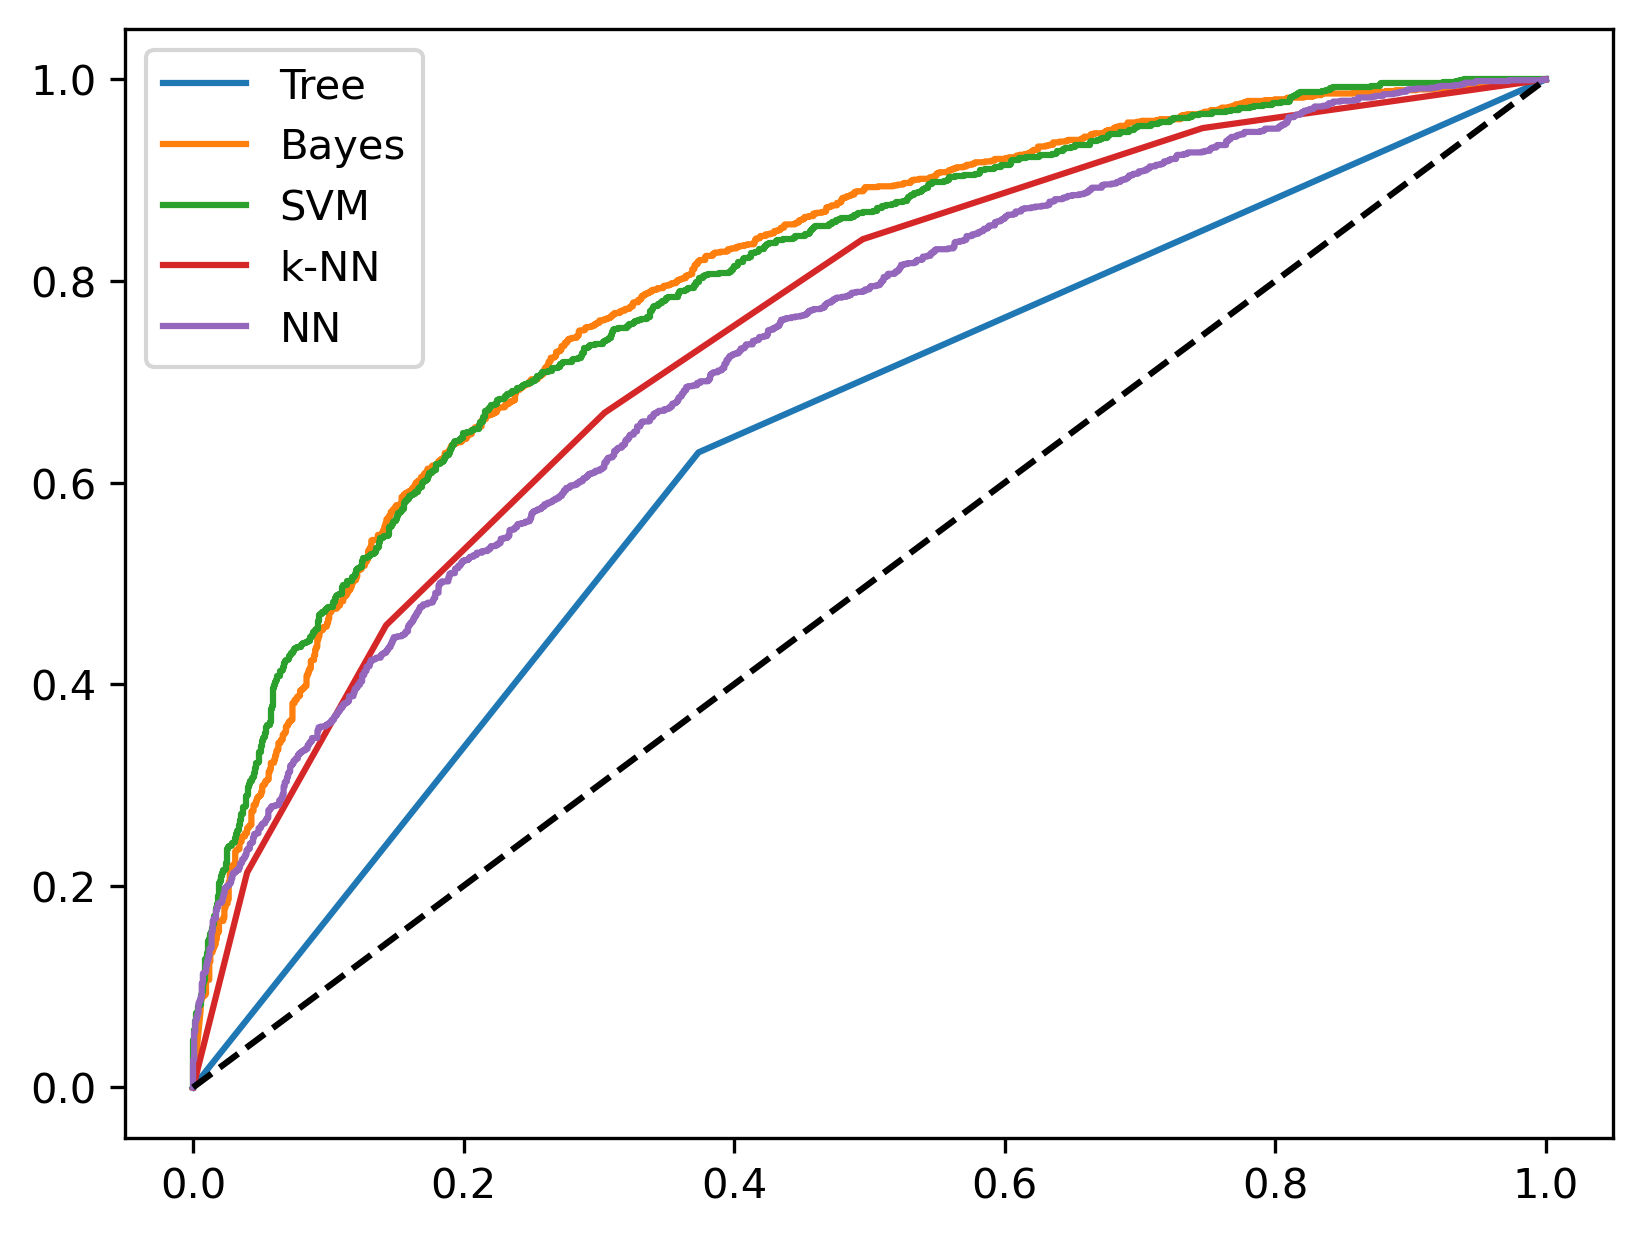
\includegraphics[width=0.90\textwidth]{images3/ROC_Curve_Rankeds.png}
    \caption{Krzywe ROC dla zbioru A}
    \label{fig:roc_curve_a}
\end{figure}

\begin{figure}[H]
    \centering
    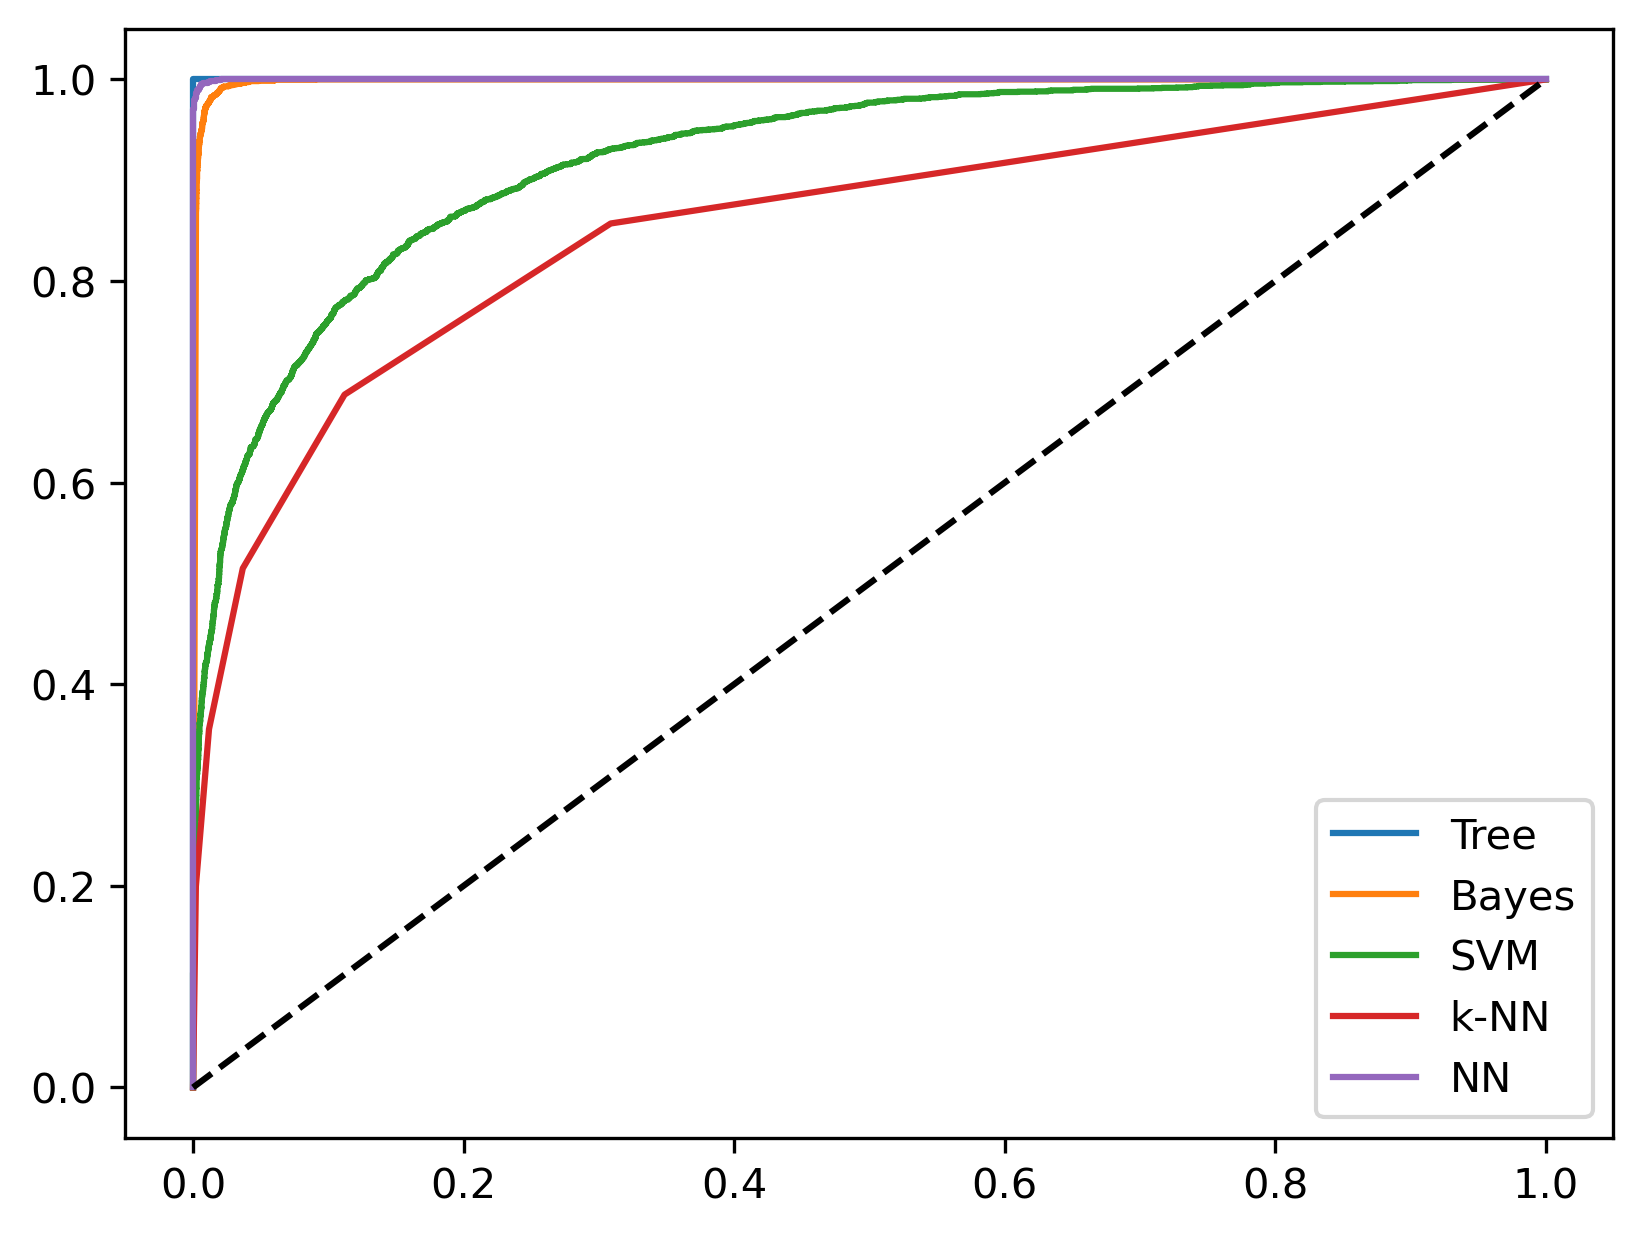
\includegraphics[width=0.90\textwidth]{images3/ROC_Curve_Rain.png}
    \caption{Krzywe ROC dla zbioru B}
    \label{fig:roc_curve_b}
\end{figure}

\begin{figure}[H]
    \centering
    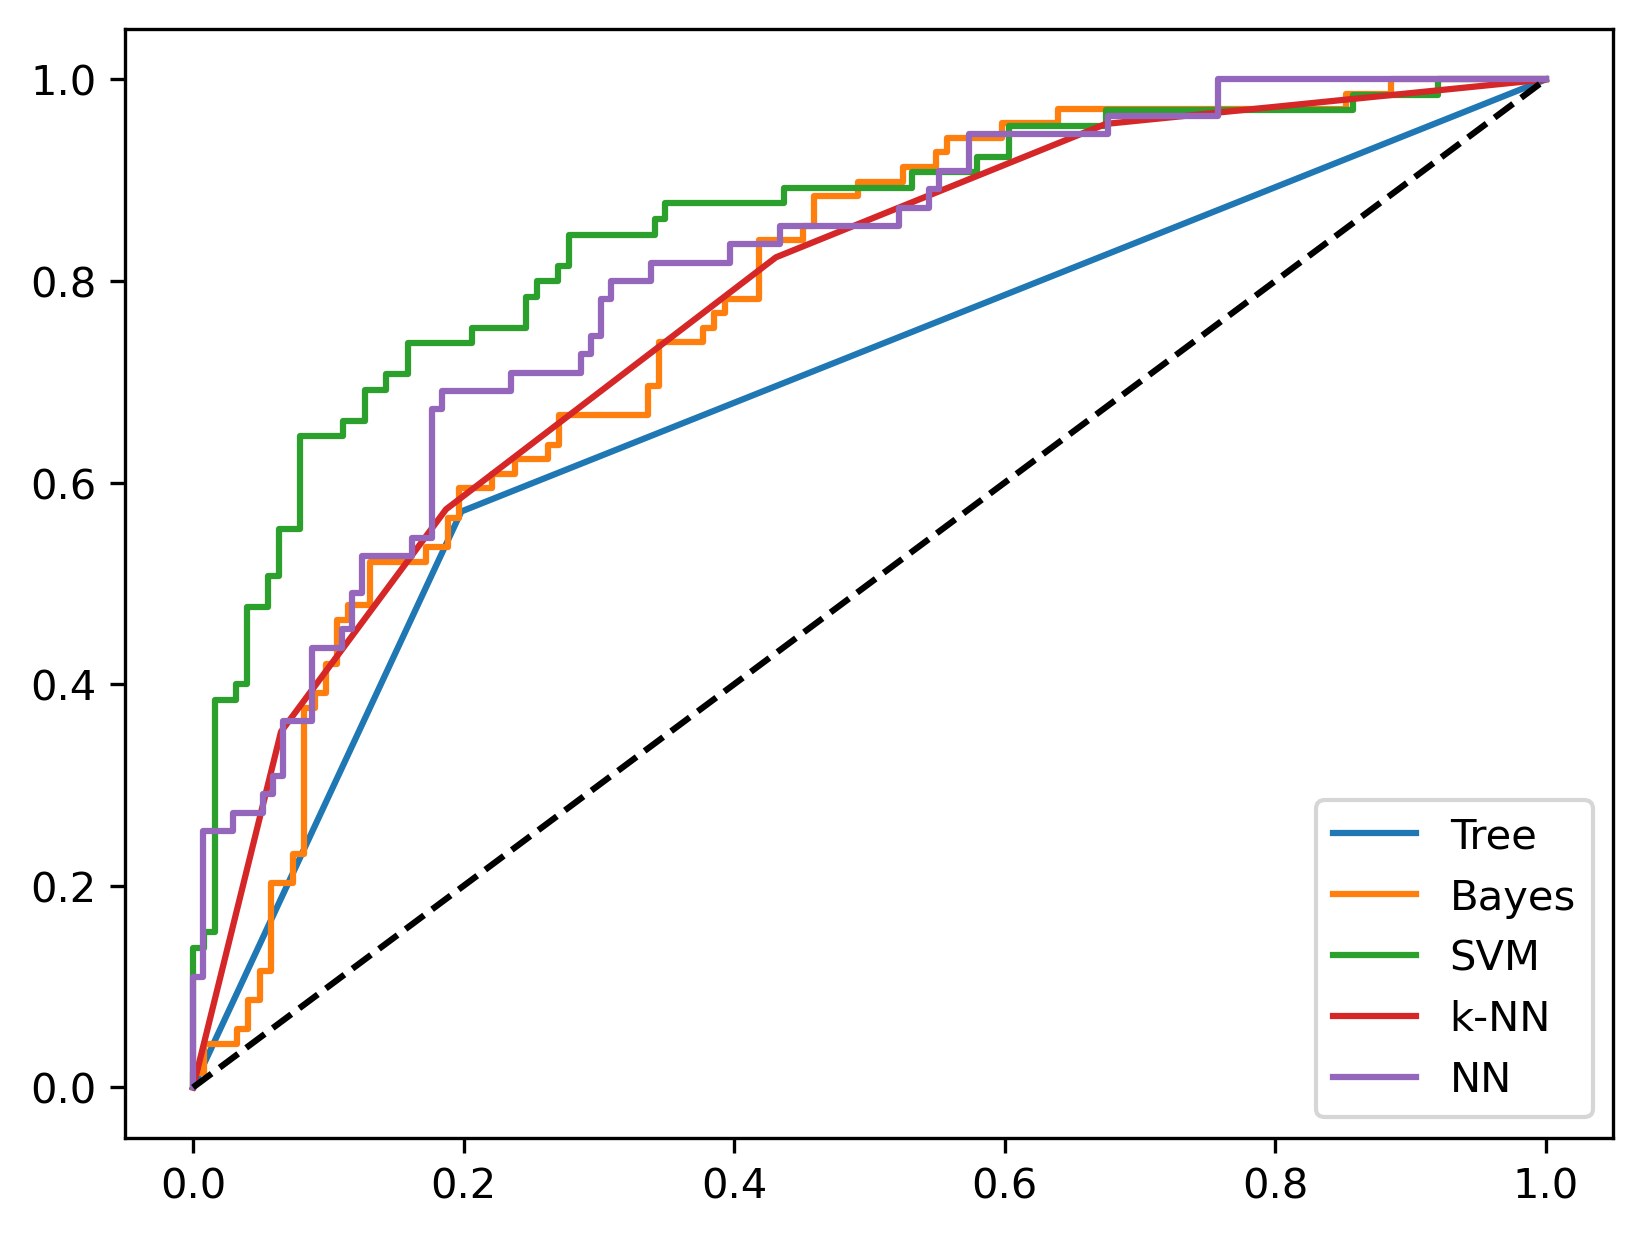
\includegraphics[width=0.90\textwidth]{images3/ROC_Curve_Diabetes.png}
    \caption{Krzywe ROC dla zbioru C}
    \label{fig:roc_curve_c}
\end{figure}

%%%%%%%%%%%%%%%%%%%%%% Krzywe uczenia się

\subsection{Krzywe uczenia się}
Kolejną częścią ewaluacji modelu było wyznaczenie krzywych uczenia się metod klasyfikacji. Wykres ten prezentuje proces zdobywania informacji przez klasyfikator w czasie. Dzięki temu określić można szybkość, z jaką dana metoda "uczy się".
Dla każdego zestawu danych wygenerowane zostały wykresy porównujące wyniki na zbiorze treningowym oraz testowym. Każdy z klasyfikatorów był trenowany kolejno na 60, 65, 70, 75, 80, 85 i 90 procentach całego zbioru danych.

\begin{figure}[H]
    \centering
    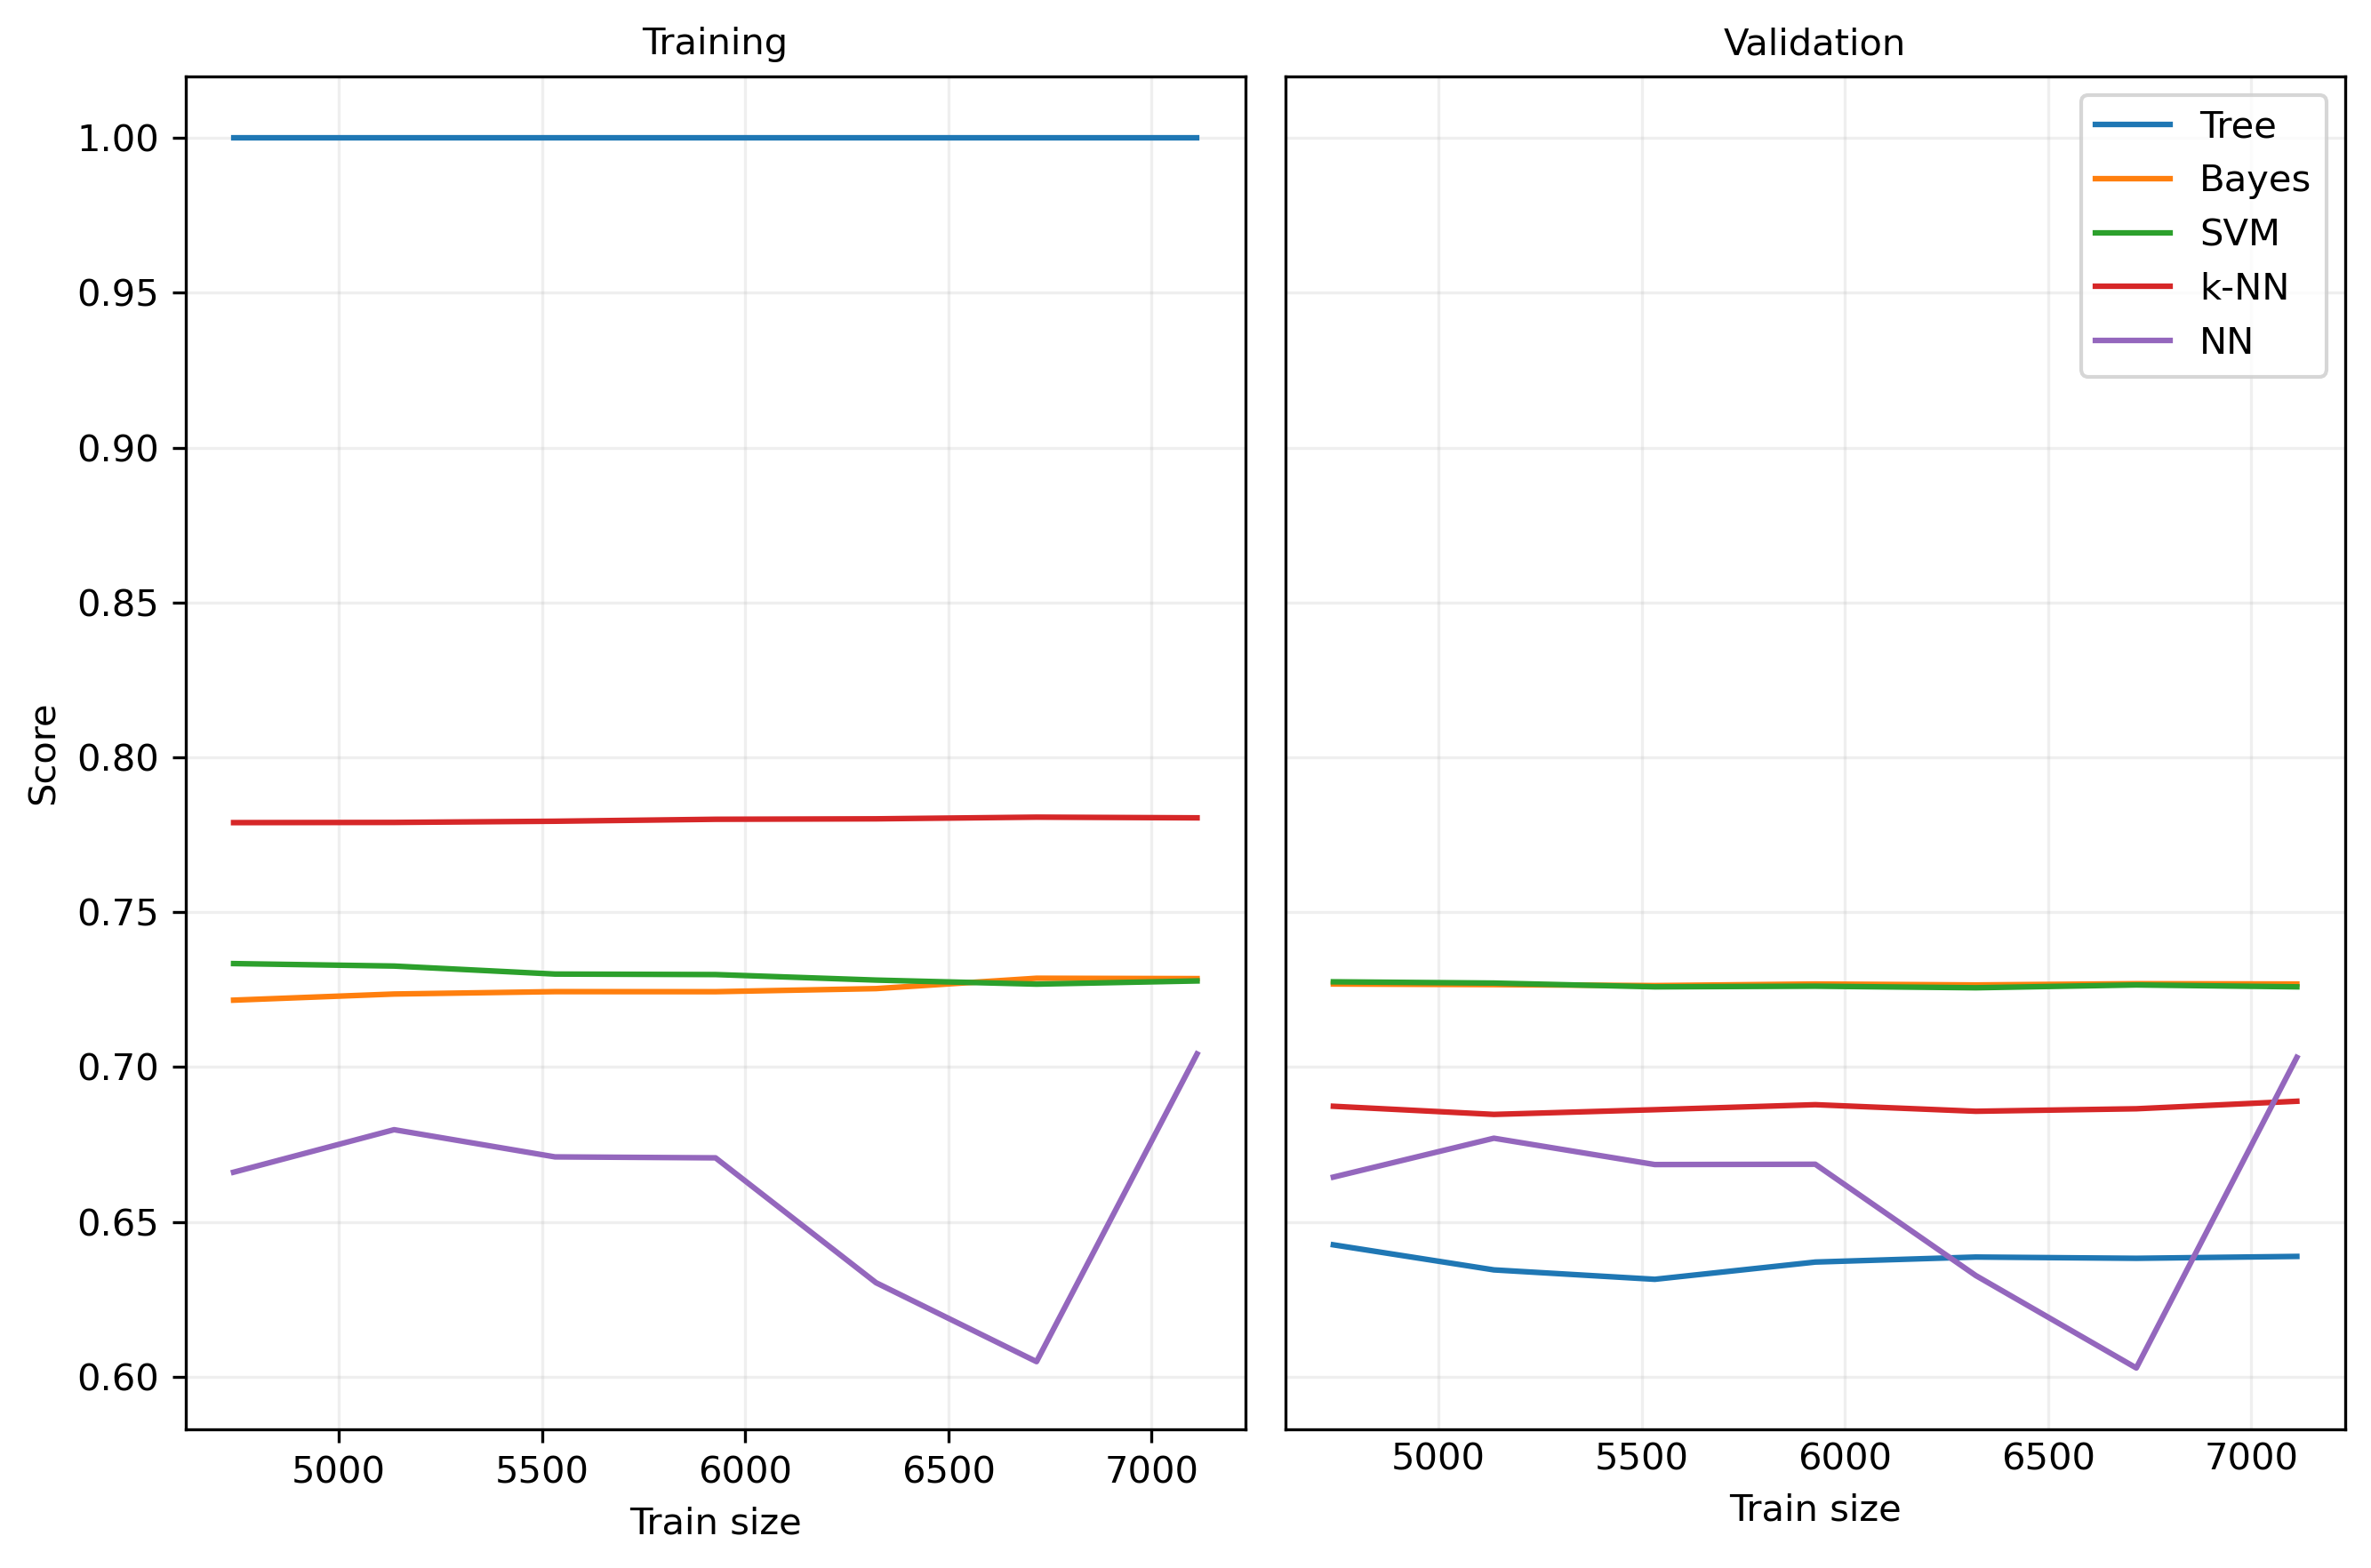
\includegraphics[width=\textwidth]{images3/learning_curves/learning_curve_Rankeds.png}
    \caption{Zestawienie krzywych dla wszystkich klasyfikatorów, dla zbioru A}
    \label{fig:learning_curve_a}
\end{figure}

\begin{figure}[H]
    \centering
    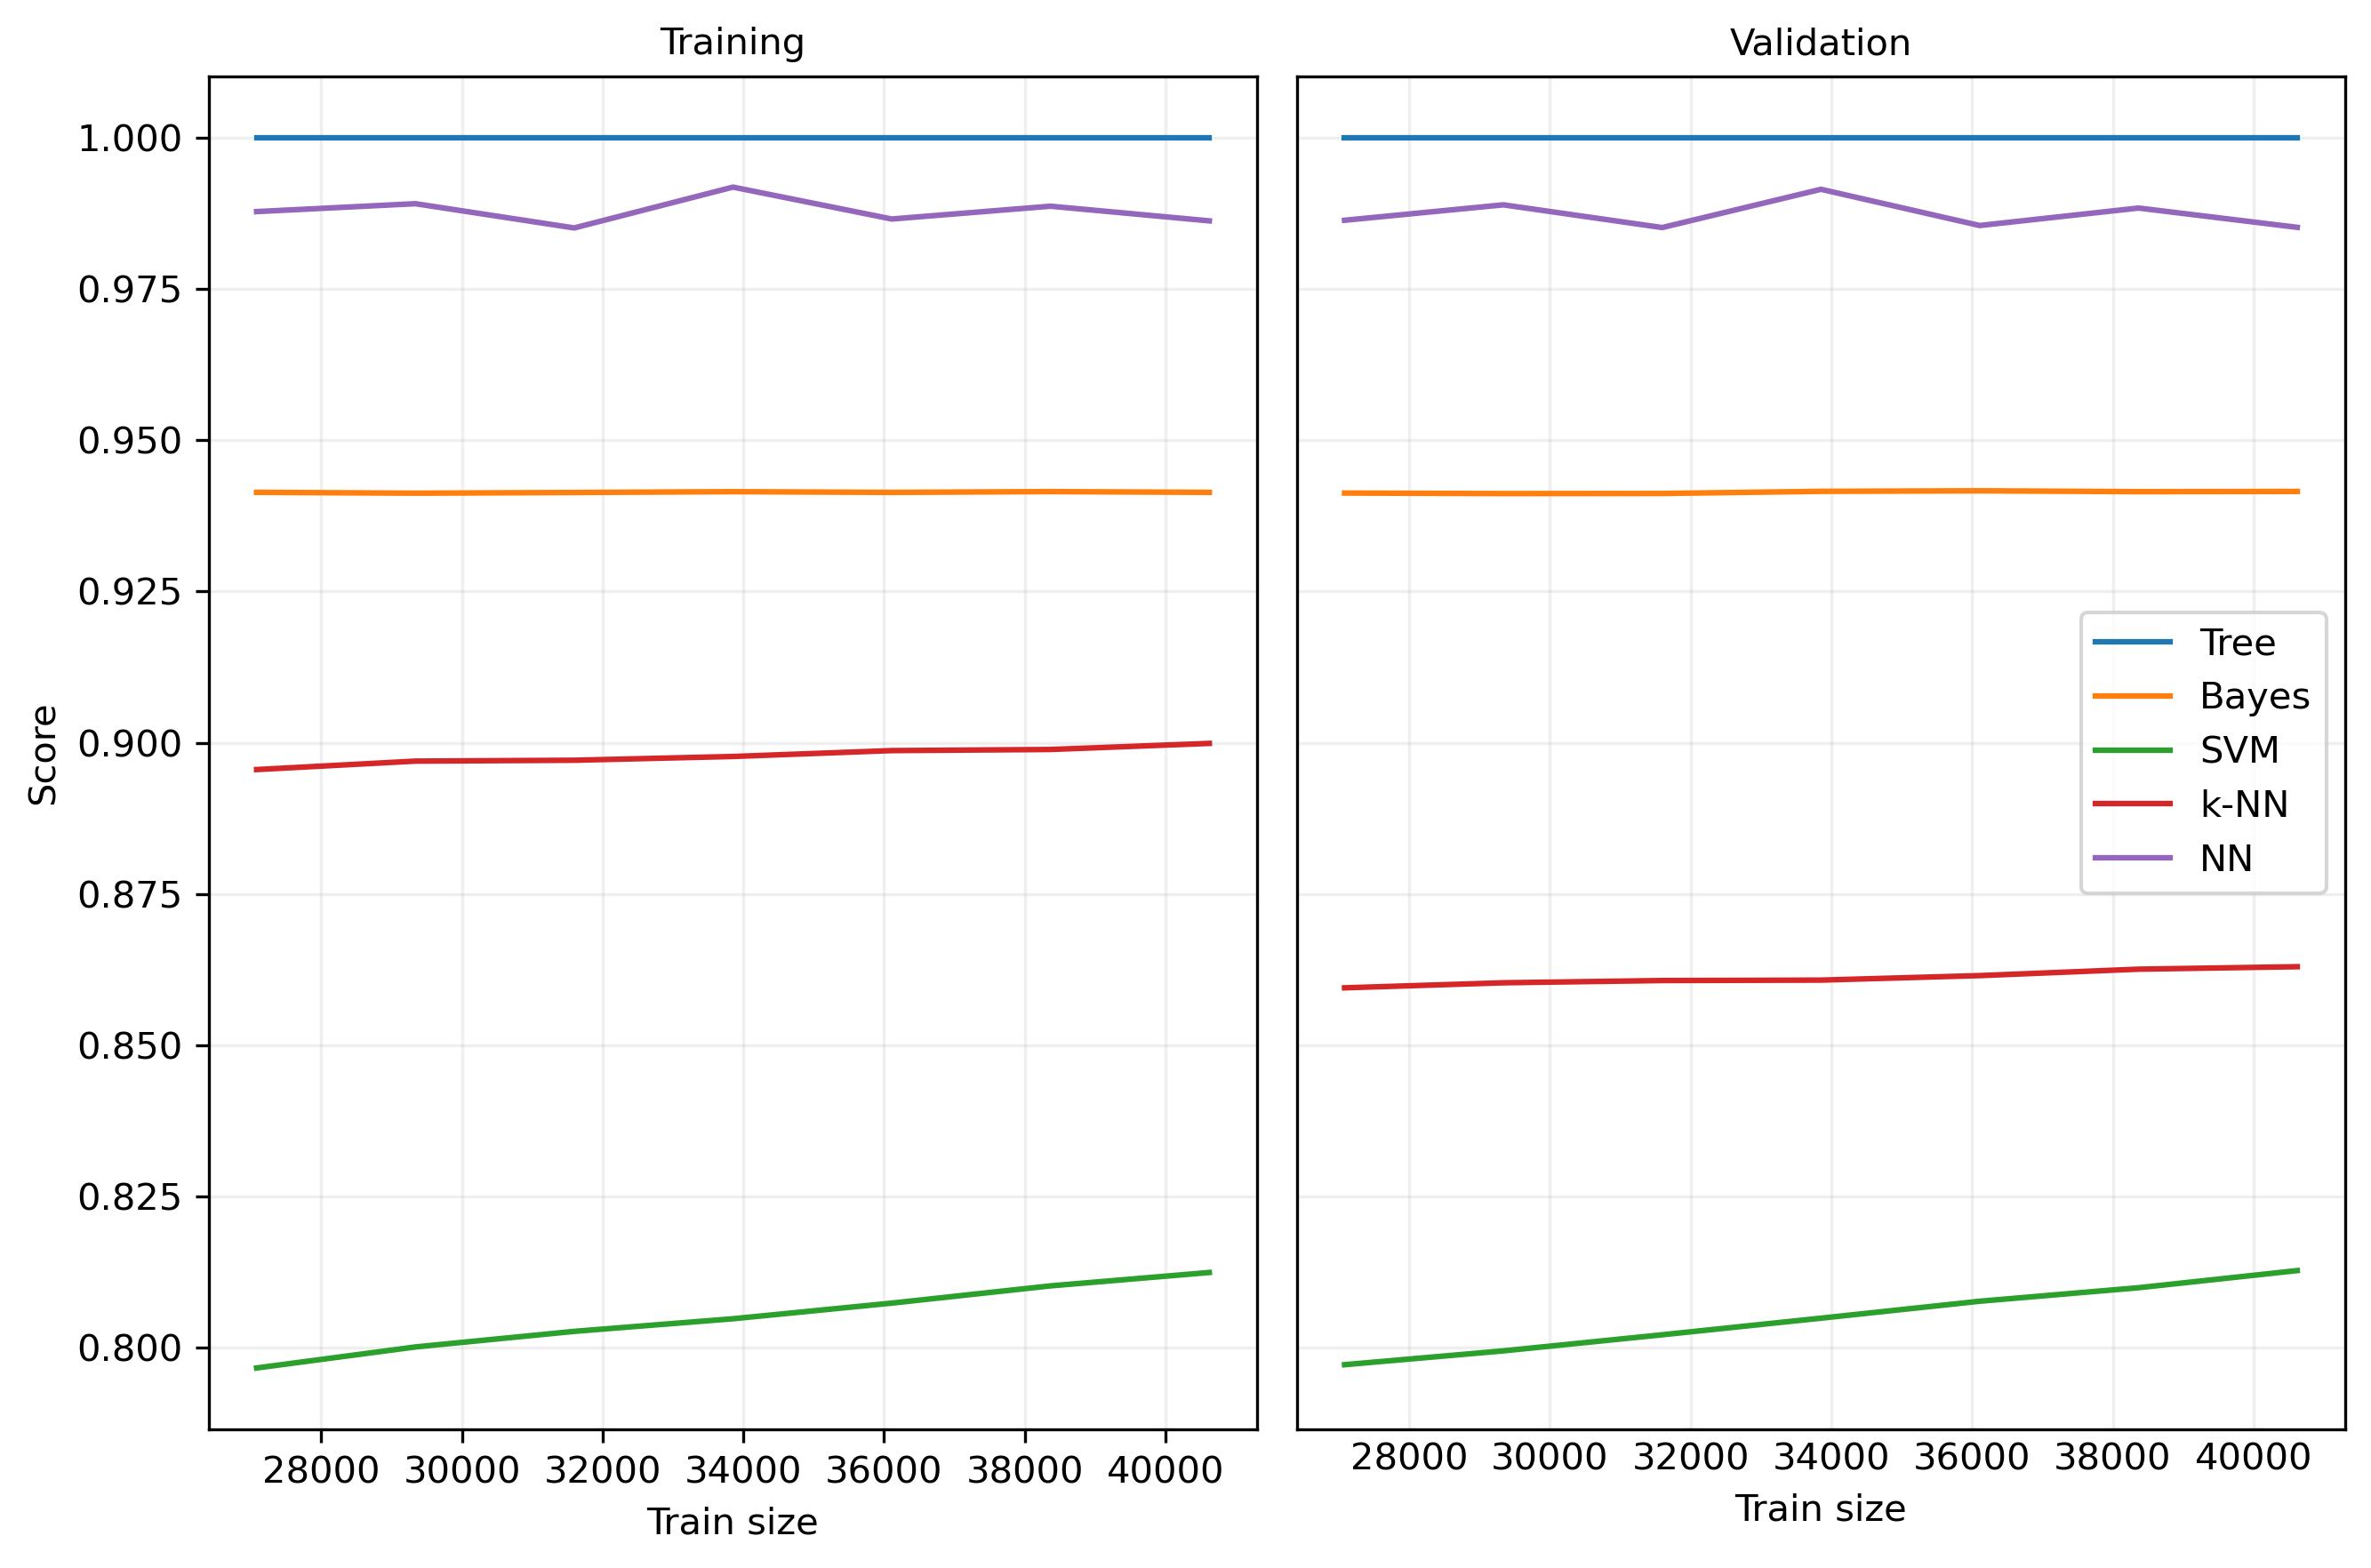
\includegraphics[width=\textwidth]{images3/learning_curves/learning_curve_Rain.png}
    \caption{Zestawienie krzywych dla wszystkich klasyfikatorów, dla zbioru B}
    \label{fig:learning_curve_b}
\end{figure}

\begin{figure}[H]
    \centering
    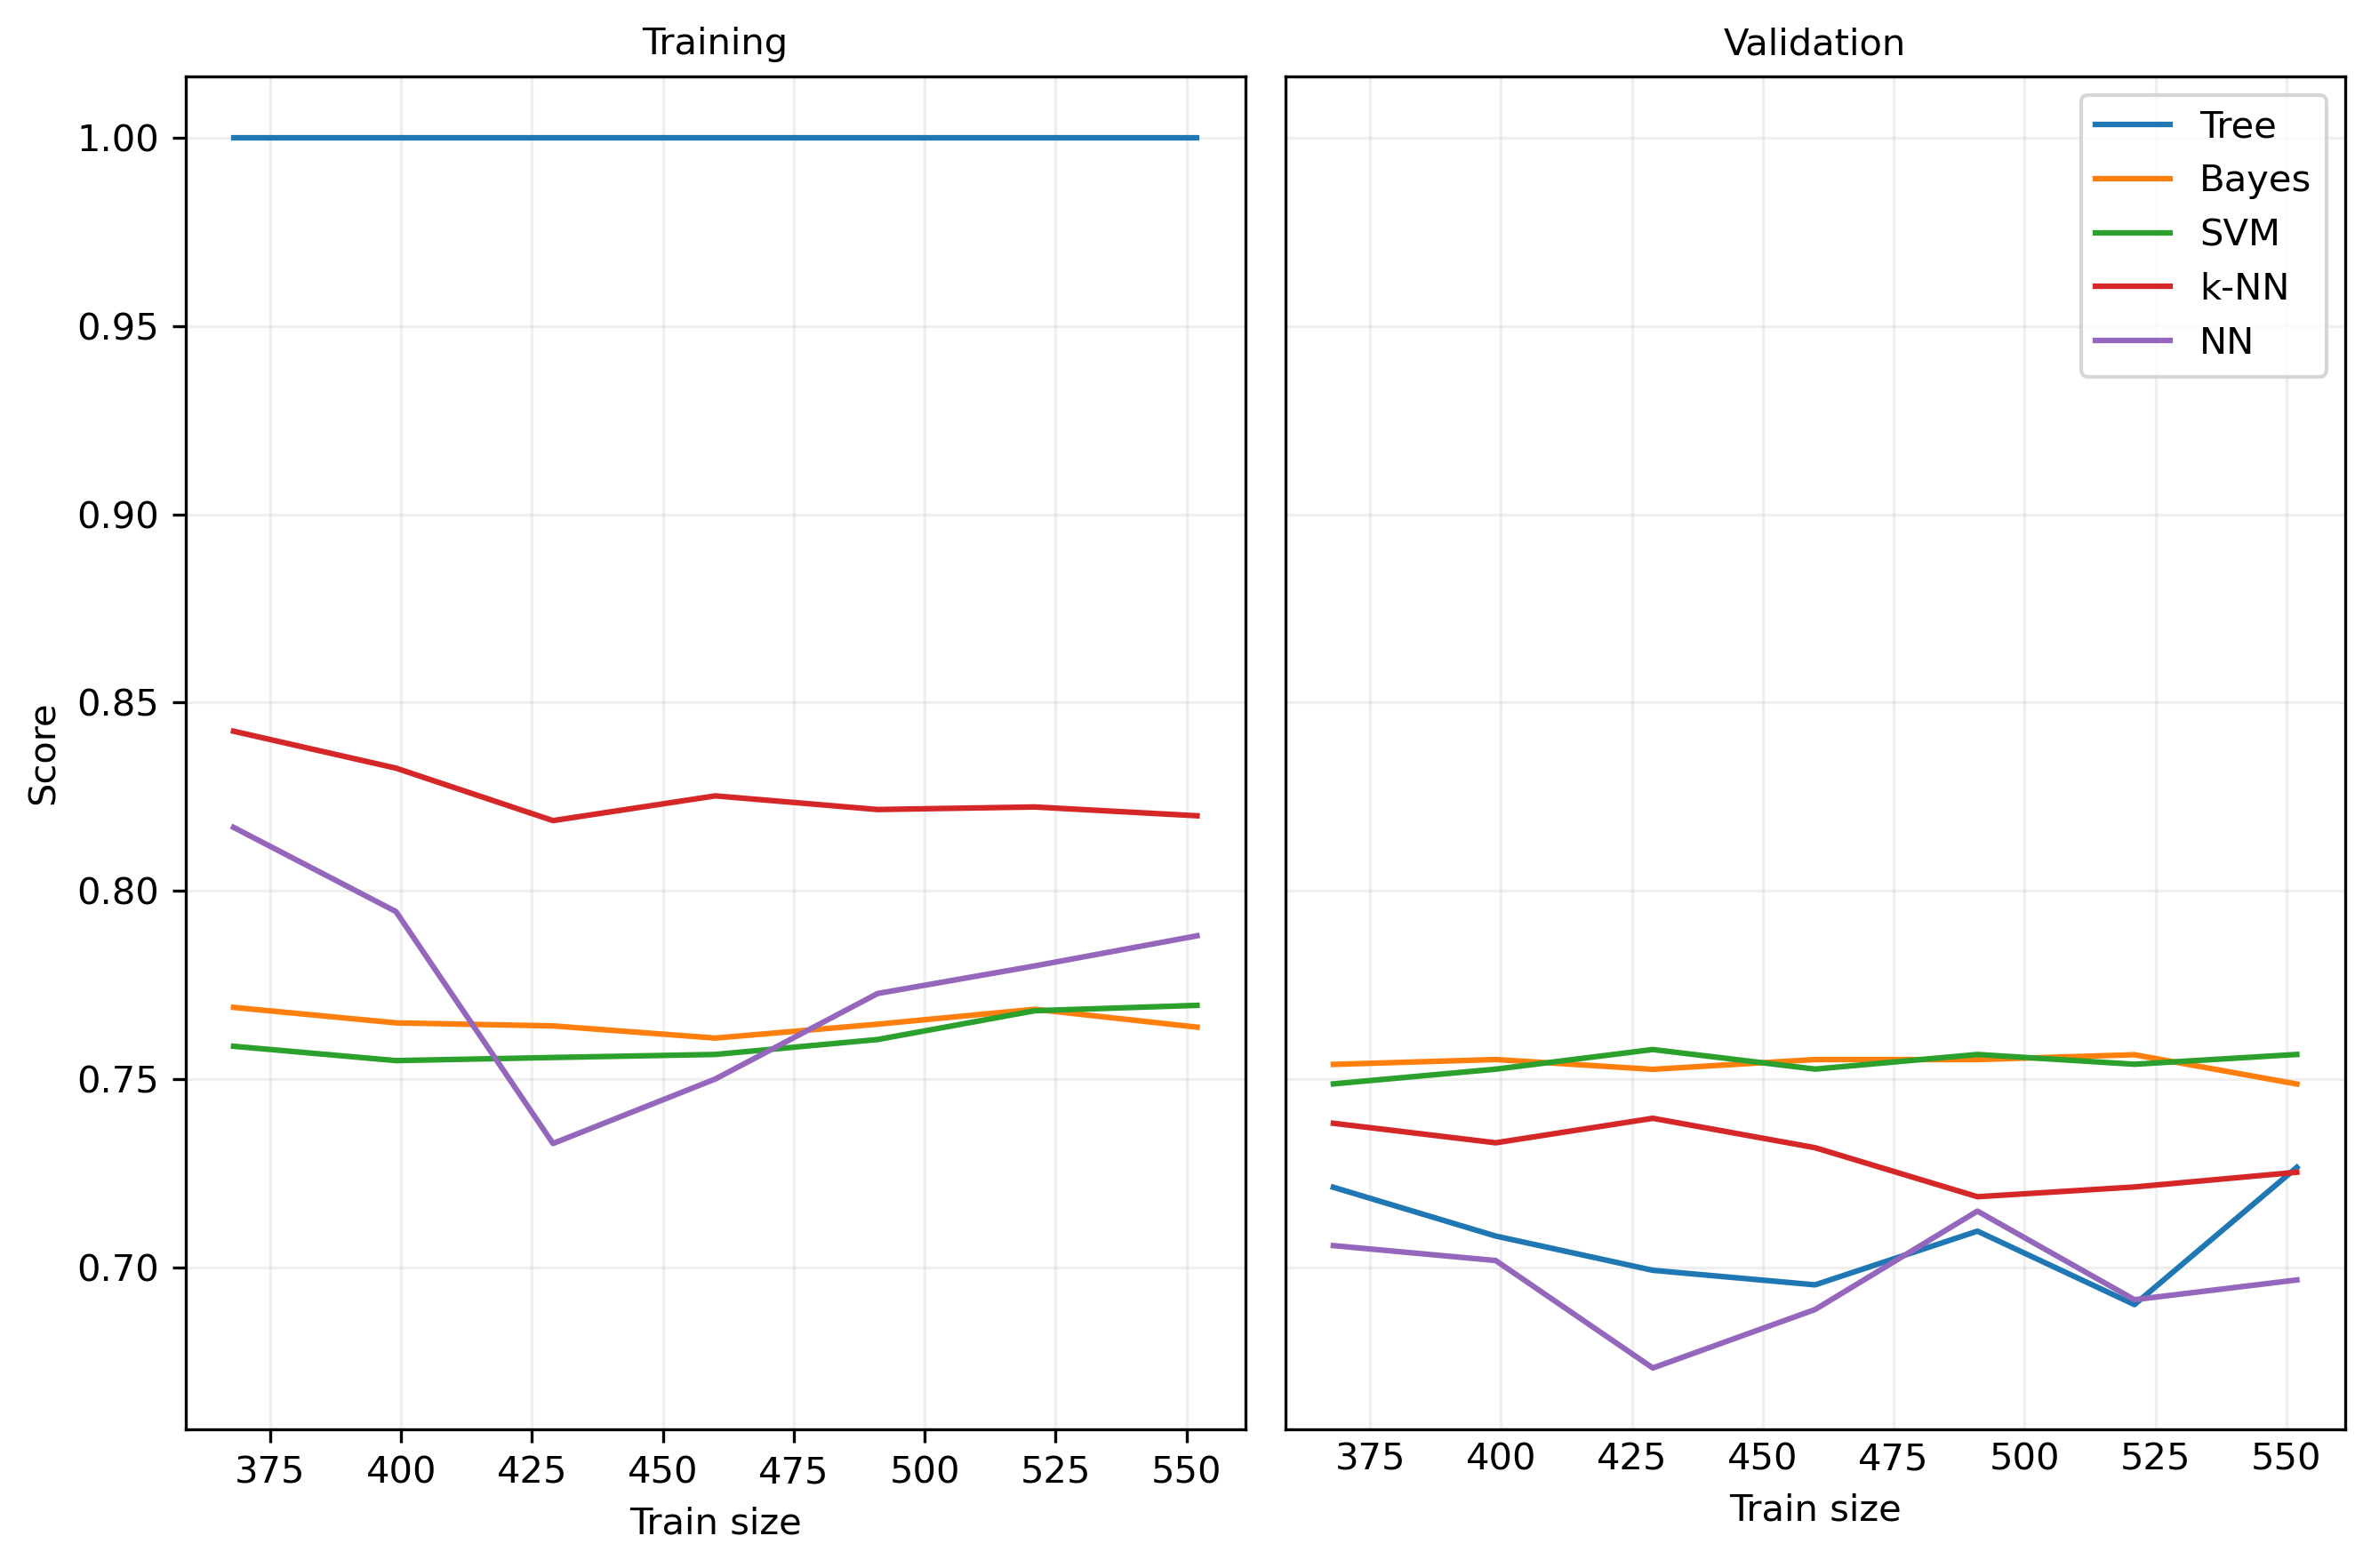
\includegraphics[width=\textwidth]{images3/learning_curves/learning_curve_Diabetes.png}
    \caption{Zestawienie krzywych dla wszystkich klasyfikatorów, dla zbioru C}
    \label{fig:learning_curve_c}
\end{figure}

% \subsection{Analiza jakości klasyfikacji}
% Ostatnim etapem ewaluacji była ocena jakości klasyfikacji wszystkich metod. 
% %jak się ocenia jakość
% Na podstawie otrzymanych wyników przygotowane zostało ich porównanie.


%%%%%%%%%%%%%%%%%%%%%%%%%%%%%%%%%%%%%%%%%%%% EWALUACJA ALGORYTMÓW SKUPIEŃ

\section{Ewaluacja modeli analizy skupień}
Zadanie 2 wymagało stworzenia modelu analizy skupień opartego o następujące metody:

\begin{enumerate}
    \item Algorytm EM,
    \item Algorytm k-średnich,
    \item Algorytm hierarchiczne aglomeracyjnego,
    \item Metoda gęstościowej DBSCAN,
    \item Metoda optics.
\end{enumerate}

Ocenie poddane zostały wyznaczone w ramach danych metod skupienia.

\subsection{Analiza wyznaczonych skupień}
Ewaluacja modelu analizy skupień zakładała po pierwsze sprawdzenie, wyznaczonych różnymi metodami, liczby skupień przyjmowanych w algorytmach. Do tego celu został wykorzystana metoda łokcia która polega na wykreśleniu zmiany w funkcji liczby skupień i wybraniu krzywej jako liczby używanych skupień oraz metoda statystyki luk która określa liczbę klastrów w zbiorze danych. Następnie wygenerowane skupienia zostały poddane analizie jakości. Ze względu na specyfikę zbiorów danych - brak etykiet - wykorzystane zostały następujące miary wewnętrzne:

\begin{itemize}
    \item Silhouette - jest miarą podobieństwa obiektu do własnego skupienia w porównaniu do innych skupień. Metoda silhouette ma przedział od -1 do +1, gdzie wysoka wartość wskazuje, że obiekt jest dobrze dopasowany do własnego klastra i słabo dopasowany do sąsiednich klastrów. Jeśli wiele punktów ma niską lub ujemną wartość, konfiguracja grupowania może mieć za dużo lub za mało klastrów.

    \item Calinski-Harabasz - metoda ta używa grupowania k-średnich, aby uzyskać wyniki  dla różnych wartości k. Przebiegi k-średnich są losowo inicjowane i dlatego muszą być uruchamiane wiele razy, aby zapewnić optymalne grupowanie.
    \item Davies-Bouldin - jest to metoda w której sprawdzanie poprawności grupowania odbywa się przy użyciu ilości cech charakterystycznych dla zestawu danych.
\end{itemize}

\subsection{Analiza zbioru danych A - "Mall Customer Segmentation"}
\begin{figure}[H]
    	\centering
    	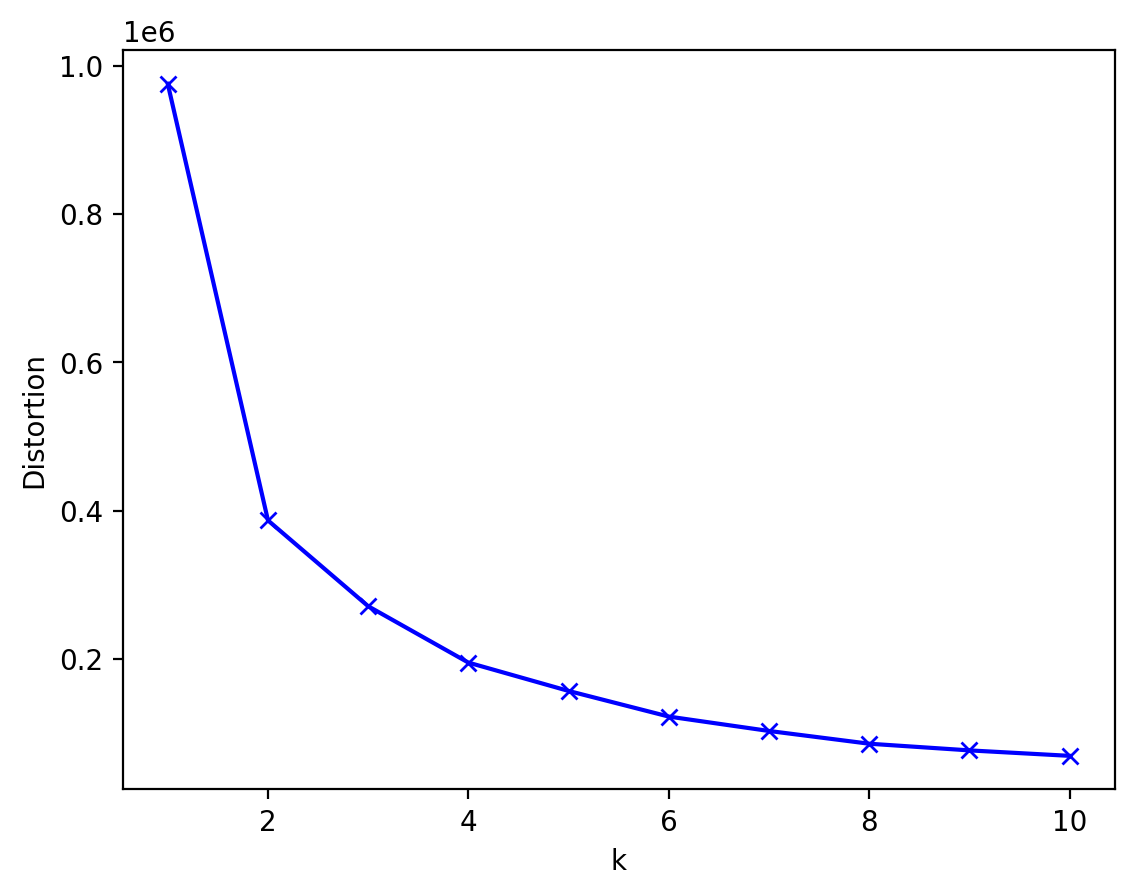
\includegraphics[width=0.67\textwidth]{images2/elbow_Customer.png}
    	\caption{Metoda "łokcia" dla zbioru danych A}
    	\label{silh_a}
\end{figure}
\begin{figure}[H]
    	\centering
    	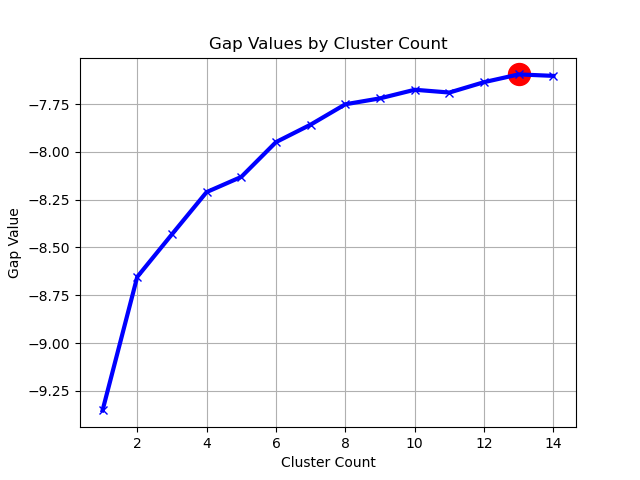
\includegraphics[width=0.67\textwidth]{images3/GAP1_13.png}
    	\caption{Metoda statystyki luk dla zbioru danych A}
    	\label{silh_b}
\end{figure}
\begin{table}[H]
\centering
\caption{Wartości metryk ewaluacyjnych dla zbioru A}
\label{tab:silh_a}
\begin{tabular}{|l|c|c|c|c|}
\hline
\multicolumn{1}{|c|}{\textbf{klaster}} & \textbf{Silhouette} & \textbf{Calinski-Harabasz} & \textbf{Davies–Bouldin}  \\ \hline
2  & 0.479 & 301.014 & 0.765  \\ \hline
3 & 0.374 & 255.565 & 0.900  \\ \hline
4 & 0.422 & 260.833 & 0.858  \\ \hline
5 & 0.421 & 253.831 & 0.866  \\ \hline
6 & 0.410 & 269.849 & 0.809  \\ \hline
7 & 0.408 & 272.036 & 0.773  \\ \hline
8 & 0.405 & 283.170 & 0.816  \\ \hline
9 & 0.395 & 277.426 & 0.822  \\ \hline
10 & 0.388 & 275.874 & 0.868  \\ \hline
\end{tabular}
\end{table}

\begin{figure}[H]
    	\centering
    	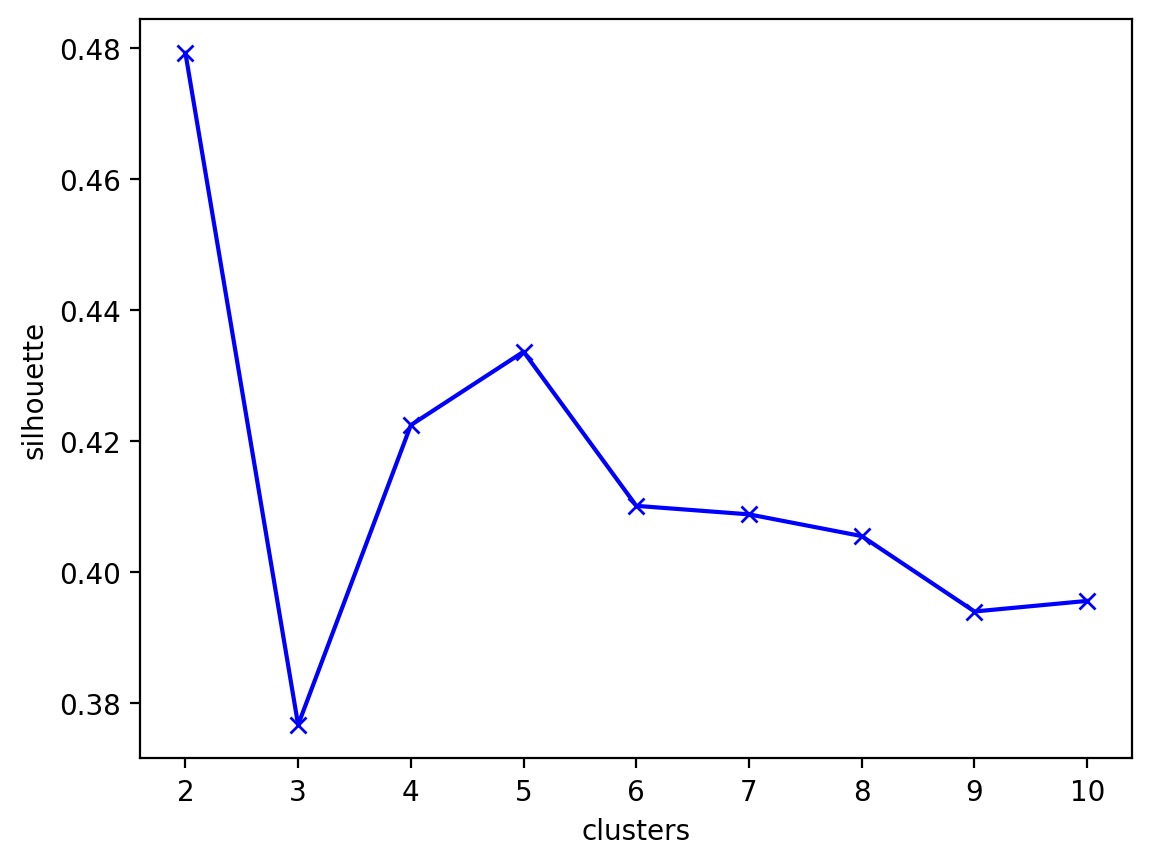
\includegraphics[width=0.67\textwidth]{images3/silhouette_Customer.png}
    	\caption{Metoda Silhouette dla zbioru danych A}
    	\label{silh_bs}
\end{figure}

\begin{figure}[H]
    	\centering
    	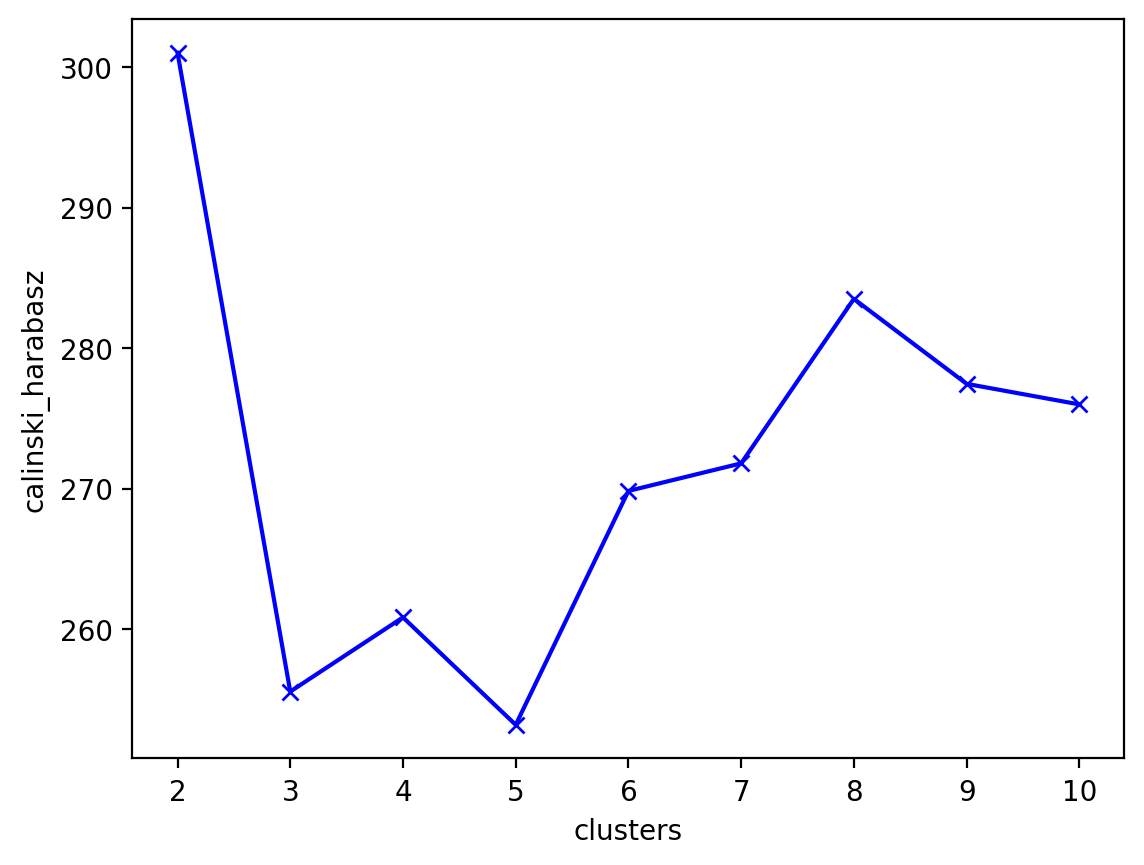
\includegraphics[width=0.67\textwidth]{images3/calinski_harabasz_Customer.png}
    	\caption{Metoda Calinski-Harabasz dla zbioru danych A}
    	\label{silh_bh}
\end{figure}

\begin{figure}[H]
    	\centering
    	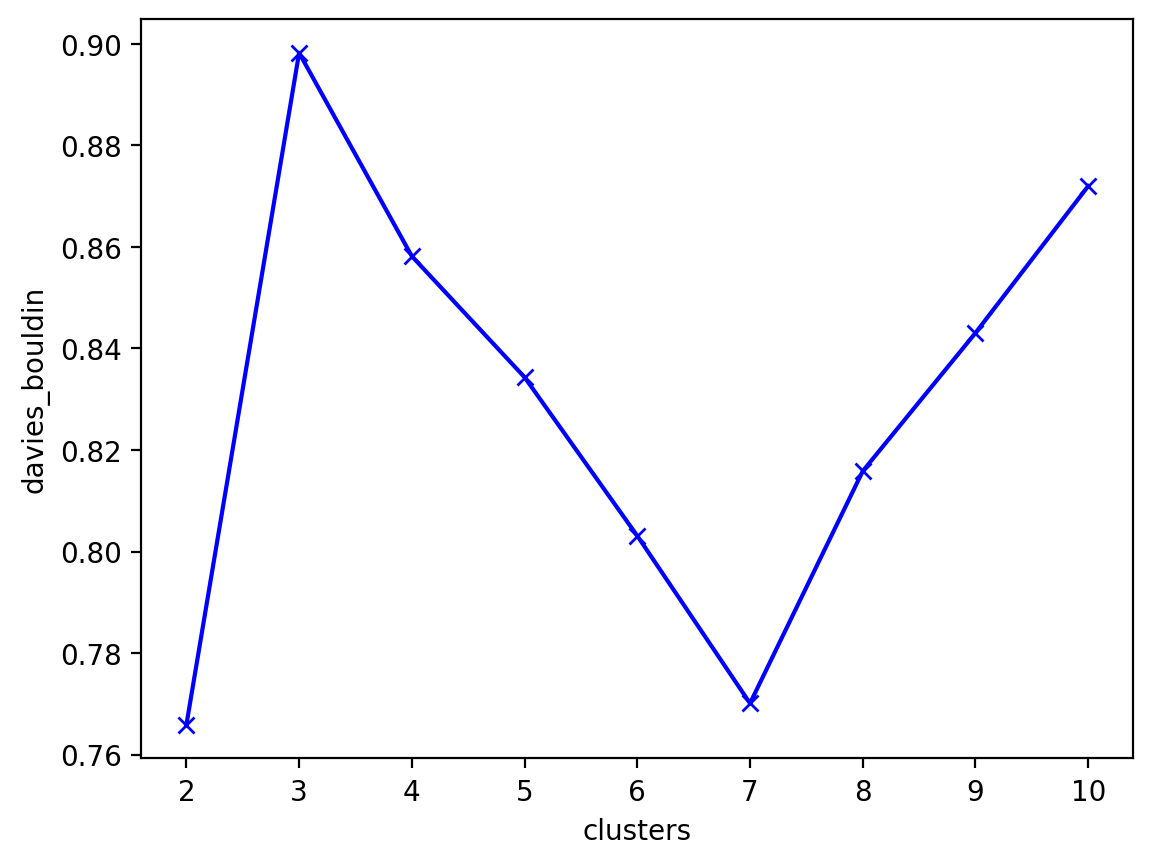
\includegraphics[width=0.67\textwidth]{images3/davies_bouldin_Customer.png}
    	\caption{Metoda Davies-Bouldin dla zbioru danych A}
    	\label{silh_bd}
\end{figure}

\subsection{Analiza zbioru danych B - "Red Wine Quality"}
\begin{figure}[H]
    	\centering
    	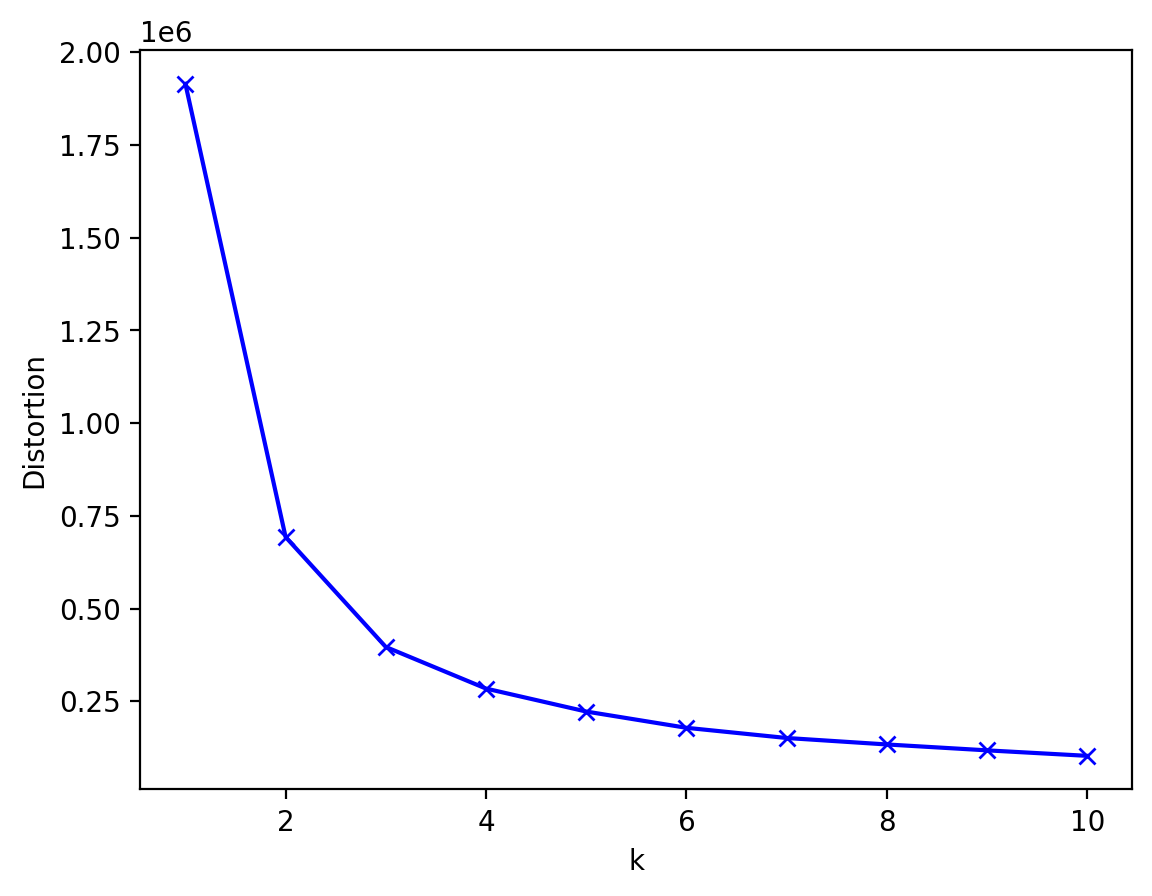
\includegraphics[width=0.67\textwidth]{images2/elbow_Wines.png}
    	\caption{Metoda "łokcia" dla zbioru danych B}
    	\label{silh_bk}
\end{figure}
\begin{figure}[H]
    	\centering
    	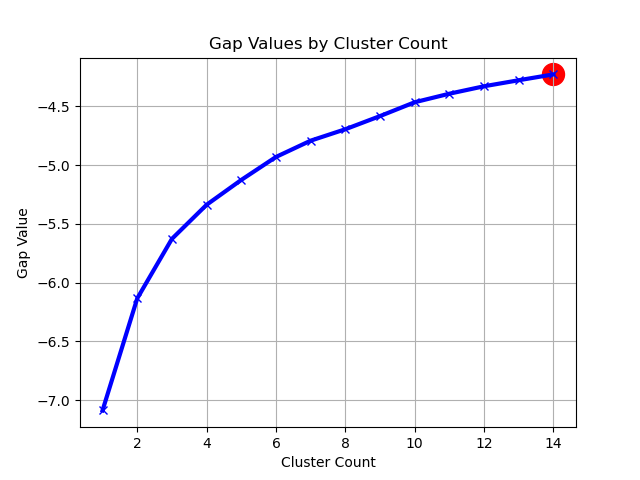
\includegraphics[width=0.67\textwidth]{images3/GAP2.png}
    	\caption{Metoda statystyki luk dla zbioru danych B}
    	\label{silh_bg}
\end{figure}
\begin{table}[H]
\centering
\caption{Wartości metryk ewaluacyjnych dla zbioru B}
\label{tab:silh_b}
\begin{tabular}{|l|c|c|c|c|}
\hline
\multicolumn{1}{|c|}{\textbf{klaster}} & \textbf{Silhouette} & \textbf{Calinski-Harabasz} & \textbf{Davies–Bouldin}  \\ \hline
2  & 0.602 & 2816.875 & 0.617  \\ \hline
3 & 0.518 & 3058.177 & 0.664  \\ \hline
4 & 0.483 & 3051.568 & 0.715  \\ \hline
5 & 0.444 & 3036.735 & 0.758  \\ \hline
6 & 0.446 & 3103.100 & 0.652  \\ \hline
7 & 0.392 & 3103.871 & 0.734  \\ \hline
8 & 0.393 & 3028.415 & 0.763  \\ \hline
9 & 0.382 & 3040.573 & 0.774  \\ \hline
10 & 0.380 & 3116.814 & 0.793  \\ \hline
\end{tabular}
\end{table}

\begin{figure}[H]
    	\centering
    	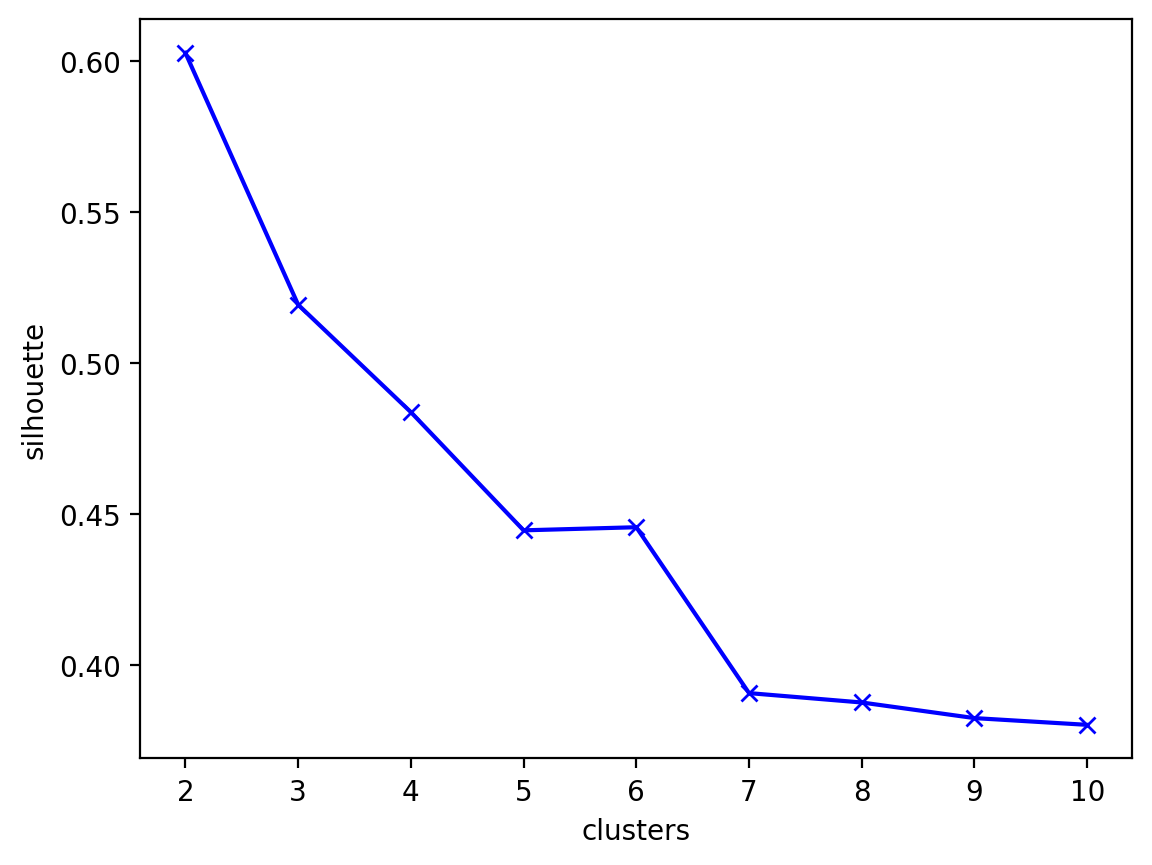
\includegraphics[width=0.67\textwidth]{images3/silhouette_Wines.png}
    	\caption{Metoda Silhouette dla zbioru danych B}
    	\label{silh_bw}
\end{figure}

\begin{figure}[H]
    	\centering
    	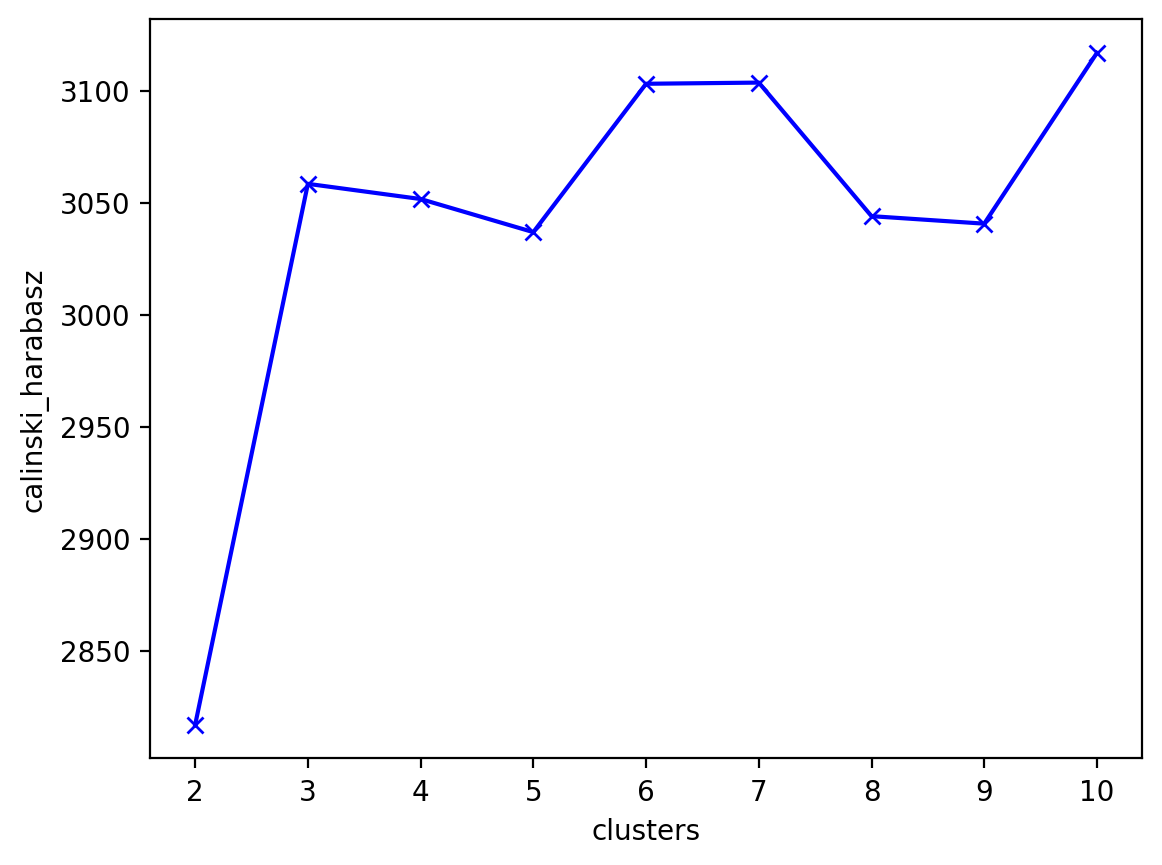
\includegraphics[width=0.67\textwidth]{images3/calinski_harabasz_Wines.png}
    	\caption{Metoda Calinski\_Harabasz dla zbioru danych B}
    	\label{silh_bhh}
\end{figure}

\begin{figure}[H]
    	\centering
    	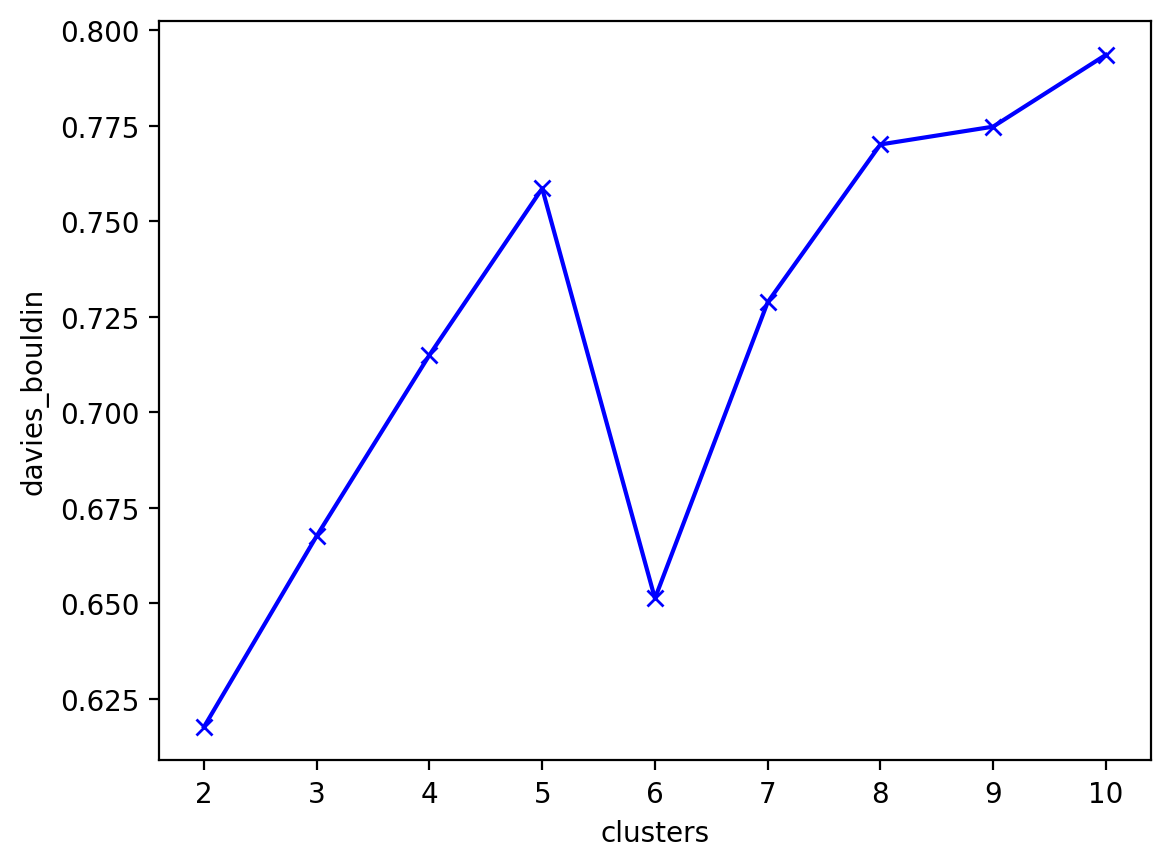
\includegraphics[width=0.67\textwidth]{images3/davies_bouldin_Wines.png}
    	\caption{Metoda Davies\_Bouldin dla zbioru danych B}
    	\label{silh_bdd}
\end{figure}

%%%%%%%%%%%%%%%%%%%%%%%%%%%%%%%%%%%%%%%%%%%% WYNIKI

\newpage
\section{Wyniki}

\begin{itemize}
    \item Dla największego zbioru danych B wszystkie klasyfikatory odznaczały się zauważalnie wyższą sprawnością, co przekładało się  na wyniki uzyskiwane na zbiorze testowym. Algorytm drzew decyzyjnych nie popełnił błędu podczas klasyfikacji danych na tym zbiorze.
    \item Algorytm sztucznej sieci neuronowej popełnia zdecydowanie więcej błędów pierwszego rodzaju niż inne algorytmy. Jest to widoczne w Czułości, której wartość jest zawsze wysoka dla tego algorytmu. Dla dużego zbioru danych algorytm Bayesa także popełnił więcej błędów pierwszego rodzaju.
    \item Na krzywych ROC widoczne jest, że algorytm drzew decyzyjnych najlepiej sobie radzi dla dużych zbiorów - jego pole zauważalnie maleje przy zbiorach A oraz C. W przypadku algorytmów maszyny wektorów nośnych oraz k-nn większa liczba przypadków treningowych nie wpływa tak zauważalnie na poprawę pola pod krzywą. 
    \item Na postawie krzywych uczenia można zaobserwować, że zjawisko niedouczenia wystąpiło w przypadku zbioru danych A o małej wielkości przy metodach drzew decyzyjnych oraz k najbliższych sąsiadów; Dla najmniejszego zbioru C wystąpiło również dla metody sieci neuronowej, a także w mniejszym stopniu dla naiwnego Bayesa oraz wektorów; Dla największego zbioru B jedynie metoda k najbliższych sąsiadów miała niższą sprawność dla danych testowych niż treningowych.
    \item Wszystkie przetestowane metody wyboru optymalnej liczby klastrów wskazały podobne wyniki.
    \item Dla dużych zbiorów danych najlepszymi metodami do oceny liczby skupień jest metoda łokcia oraz metoda luki.
\end{itemize}

% %%%%%%%%%%%%%%%%%%%%%%%%%%%%%%%%%%%%%%%%%%%% BIBLIOGRAFIA XD

% \newpage
% \begin{thebibliography}{0}

%     \bibitem{ClusteringQuality}
%     \textsl{Prelekcja Christiana Henniga dotycząca oceny jakości klasteryzacji, \url{https://www.youtube.com/watch?v=Mf6MqIS2ql4}}
    
% \end{thebibliography}

\end{document}
